%%%%%%%%%%%%%%%%%%%%%%%%%%%%%%%%%%%%%%%%%
% The Legrand Orange Book
% LaTeX Template
% Version 3.1 (February 18, 2022)
%
% This template originates from:
% https://www.LaTeXTemplates.com
%
% Authors:
% Vel (vel@latextemplates.com)
% Mathias Legrand (legrand.mathias@gmail.com)
%
% License:
% CC BY-NC-SA 4.0 (https://creativecommons.org/licenses/by-nc-sa/4.0/)
%
% Compiling this template:
% This template uses biber for its bibliography and makeindex for its index.
% When you first open the template, compile it from the command line with the
% commands below to make sure your LaTeX distribution is configured correctly:
%
% 1) pdflatex main
% 2) makeindex main.idx -s indexstyle.ist
% 3) biber main
% 4) pdflatex main x 2
%
% After this, when you wish to update the bibliography/index use the appropriate
% command above and make sure to compile with pdflatex several times
% afterwards to propagate your changes to the document.
%
%%%%%%%%%%%%%%%%%%%%%%%%%%%%%%%%%%%%%%%%%

%----------------------------------------------------------------------------------------
%	PACKAGES AND OTHER DOCUMENT CONFIGURATIONS
%----------------------------------------------------------------------------------------

\documentclass[
	11pt, % Default font size, select one of 10pt, 11pt or 12pt
	fleqn, % Left align equations
	a4paper, % Paper size, use either 'a4paper' for A4 size or 'letterpaper' for US letter size
	%oneside, % Uncomment for oneside mode, this doesn't start new chapters and parts on odd pages (adding an empty page if required), this mode is more suitable if the book is to be read on a screen instead of printed
]{LegrandOrangeBook}


% Book information for PDF metadata, remove/comment this block if not required
\hypersetup{
	pdftitle={Title}, % Title field
	pdfauthor={Author}, % Author field
	pdfsubject={Subject}, % Subject field
	pdfkeywords={Keyword1, Keyword2, ...}, % Keywords
	pdfcreator={LaTeX}, % Content creator field
}

\addbibresource{sample.bib} % Bibliography file

\definecolor{ocre}{RGB}{26, 201, 128} % Define the color used for highlighting throughout the book

%\chapterimage{orange1.jpg} % Chapter heading image
\chapterimage{}
\chapterspaceabove{6.5cm} % Default whitespace from the top of the page to the chapter title on chapter pages
\chapterspacebelow{6.75cm} % Default amount of vertical whitespace from the top margin to the start of the text on chapter pages

%----------------------------------------------------------------------------------------

\usepackage{listings}
\usepackage{xcolor}
\usepackage{tikz}
\usepackage{tkz-graph}
\usepackage{tkz-berge}

\definecolor{codegreen}{rgb}{0,0.6,0}
\definecolor{codegray}{rgb}{0.5,0.5,0.5}
\definecolor{codepurple}{rgb}{0.58,0,0.82}
\definecolor{backcolour}{rgb}{0.95,0.95,0.92}

\lstdefinestyle{incellstyle}{
    backgroundcolor=\color{backcolour},
    commentstyle=\color{codegreen},
    keywordstyle=\color{magenta},
    numberstyle=\tiny\color{codegray},
    stringstyle=\color{codepurple},
    basicstyle=\ttfamily\footnotesize,
    breakatwhitespace=false,
    breaklines=true,
    captionpos=b,
    keepspaces=true,
    numbers=left,
    numbersep=5pt,
    showspaces=false,
    showstringspaces=false,
    showtabs=false,
    tabsize=2,
	numbers=none,
	frame=lines,
	framextopmargin=2pt,
	framexbottommargin=2pt
}

\lstdefinestyle{outcellstyle}{
    backgroundcolor=\color{white},
    commentstyle=\color{codegreen},
    keywordstyle=\color{magenta},
    numberstyle=\tiny\color{codegray},
    stringstyle=\color{codepurple},
    basicstyle=\ttfamily\footnotesize,
    breakatwhitespace=false,
    breaklines=true,
    captionpos=b,
    keepspaces=true,
    numbers=left,
    numbersep=5pt,
    showspaces=false,
    showstringspaces=false,
    showtabs=false,
    tabsize=2,
	numbers=none,
	frame=lines,
	framextopmargin=2pt,
	framexbottommargin=2pt
}

\lstset{style=incellstyle}

\lstnewenvironment{sageCell}{%
	\smallskip
	\lstset{style=incellstyle,language=Python}
}
{}

\lstnewenvironment{outCell}{%
	\smallskip
	\lstset{style=outcellstyle,language=Python}
}
{}

% \newcommand{cmd}[args][default]{def}

\newenvironment{outImage}{
	%

	\begin{samepage}
	\noindent\hrulefill
	\begin{center}
}{
	\end{center}
	\noindent\hrulefill
	\end{samepage}

	%
}

\begin{document}

%----------------------------------------------------------------------------------------
%	TITLE PAGE
%----------------------------------------------------------------------------------------

\titlepage % Output the title page
    {\makebox[\paperwidth]{}}
	% {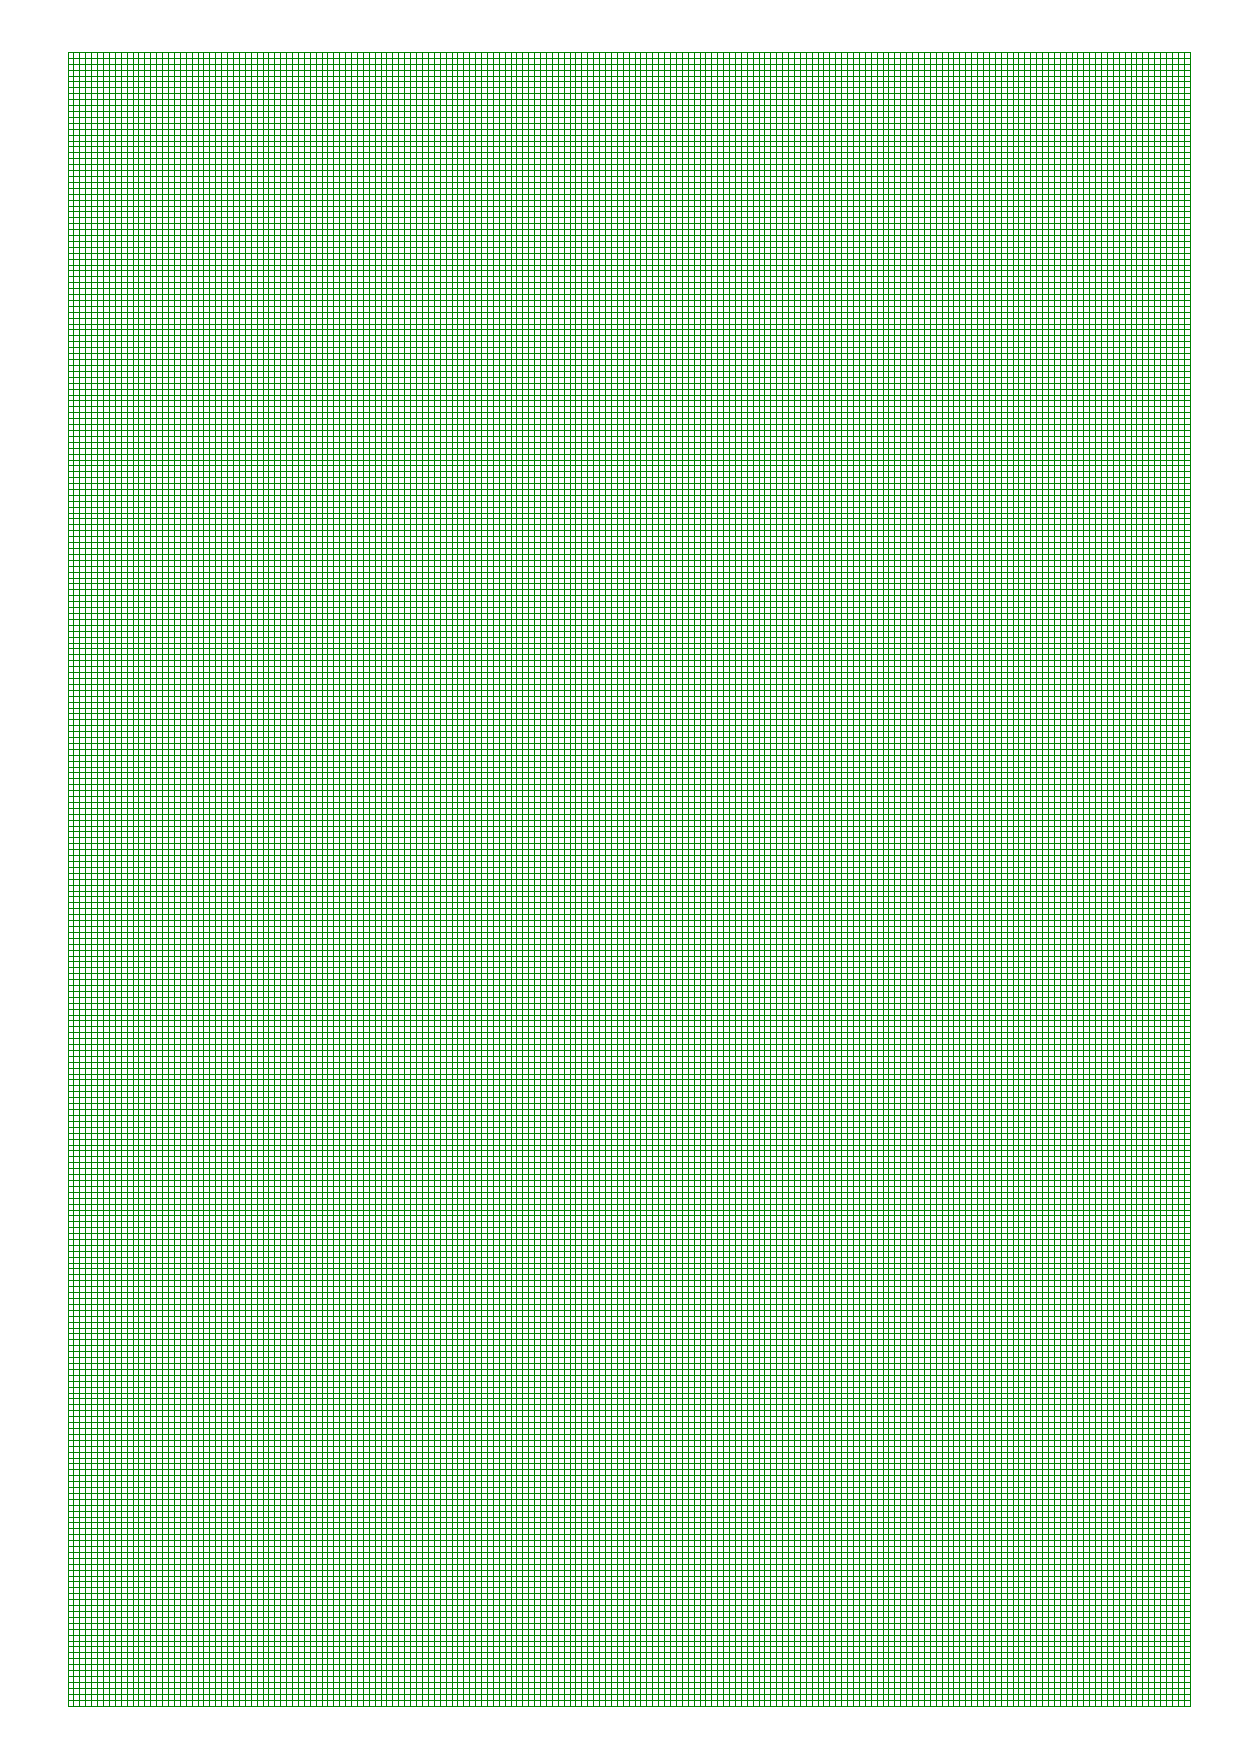
\includegraphics[width=\paperwidth]{background_green.pdf}} % Code to output the background image, which should be the same dimensions as the paper to fill the page entirely; leave empty for no background image
	{ % Title(s) and author(s)
		\centering\sffamily % Font styling
		{\Huge\bfseries Diskretna matematika 2\par} % Book title
		\vspace{16pt} % Vertical whitespace
		{\LARGE Gradiva za vaje iz diskretne matematike 2\\[1mm] Univerza v Ljubljani, Fakulteta za računalnišvo in informatiko \par} % Subtitle
		\vspace{24pt} % Vertical whitespace
		{\huge\bfseries Marko Boben\par} % Author name
	}

%----------------------------------------------------------------------------------------
%	COPYRIGHT PAGE
%----------------------------------------------------------------------------------------

\thispagestyle{empty} % Suppress headers and footers on this page

~\vfill % Push the text down to the bottom of the page

\noindent Copyright \copyright\ 2023 Marko Boben\\ % Copyright notice

% \noindent \textsc{Published by Publisher}\\ % Publisher

\noindent \textsc{\href{https://www.fri.uni-lj.si/markobob/dm2-book.pdf}{Website}}\\ % URL

\noindent Licensed under the Creative Commons Attribution-NonCommercial 4.0 License (the ``License''). You may not use this file except in compliance with the License. You may obtain a copy of the License at \url{https://creativecommons.org/licenses/by-nc-sa/4.0}. Unless required by applicable law or agreed to in writing, software distributed under the License is distributed on an \textsc{``as is'' basis, without warranties or conditions of any kind}, either express or implied. See the License for the specific language governing permissions and limitations under the License.\\ % License information, replace this with your own license (if any)

\noindent \textit{June 2023} % Printing/edition date

%----------------------------------------------------------------------------------------
%	TABLE OF CONTENTS
%----------------------------------------------------------------------------------------

\pagestyle{empty} % Disable headers and footers for the following pages

\tableofcontents % Output the table of contents

% \listoffigures % Output the list of figures, comment or remove this command if not required

% \listoftables % Output the list of tables, comment or remove this command if not required

\pagestyle{fancy} % Enable default headers and footers again

\cleardoublepage % Start the following content on a new page

\chapterimage{}
\chapterspaceabove{6.75cm} % Whitespace from the top of the page to the chapter title on chapter pages
\chapterspacebelow{7.25cm} % Amount of vertical whitespace from the top margin to the start of the
%------------------------------------------------

\chapter{Introduction}\index{Introduction}

\section{What is Sage?}

Algorithms in this Notes are implemented in Python programming language using SageMath (\url{https://www.sagemath.org}).


\begin{dBox}
SageMath is a free open-source mathematics software system licensed under the GPL.
It builds on top of many existing open-source packages: NumPy, SciPy, matplotlib, Sympy, Maxima, GAP, FLINT,
R and many more.
\end{dBox}

You can download binaries at \url{http://www.sagemath.org/download.html} for Mac, and Windows.

Note: Binaries for Windows are avaliable up to version 9.3 (late 2021).
For newer versions you will need to install it in WSL. Follow the instructions at\url{https://doc.sagemath.org/html/en/installation/index.html}.


There is also a cloud version available at https://cocalc.com/

% Using `sage -n jupyter` or running `SageMath 9.x Notebook` application (on Windows) you start jupyter notebook server on localhost:8888.

\noindent Documentation can be found at \url{https://doc.sagemath.org/html/en/index.html}.

\noindent We will moslty use \emph{graph theory} package \url{https://doc.sagemath.org/html/en/reference/graphs/index.html}

\section{Some examples of Sage Graph Theory objects and methods}

For representing undirected graphs we use the \texttt{Graph} class, while for representing directed graphs we use the \texttt{DiGraph} class.

\subsection{Undirected graphs}

Undirected graph is represented using \texttt{Graph} class.

\begin{sageCell}
    G = Graph({0:[1,2,3], 4:[0,2], 6:[1,2,3,4,5]})
\end{sageCell}
There are many methods to access the graph properties. For example, to get a list of vertices use \texttt{vertices} method.
\begin{sageCell}
    G.vertices()
\end{sageCell}
\begin{outCell}
    [0,1,2,3,4,5,6]
\end{outCell}


To display the graph, simply execute a cell with the graph variable name.
\begin{sageCell}
    G
\end{sageCell}

The output is a graphical representation of the graph. If we do not specify vertex coordinates (see below), Sage will use a spring embedder layout algorithm to compute the coordinates.
\begin{outImage}
    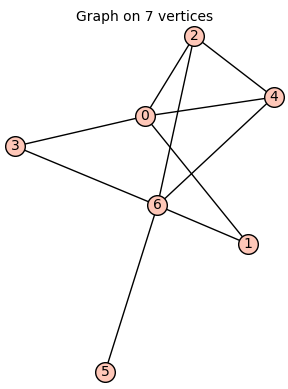
\includegraphics[width=6cm]{Images/Introduction/output_96_0.png}
\end{outImage}

If a graph is too large, it will not be displayed. In this case, or if you need to specify other display options, you can use the \texttt{plot} method. There are many options for the \texttt{plot} method, see \url{https://doc.sagemath.org/html/en/reference/plotting/sage/graphs/graph_plot.html} for details.

\medskip
For example. we can specify vertex colors using a dictionary, where keys are colors and values are lists of vertices.
\begin{sageCell}
    G.plot(vertex_colors={'red':[1],'green':[0,4]})
\end{sageCell}
\begin{outImage}
    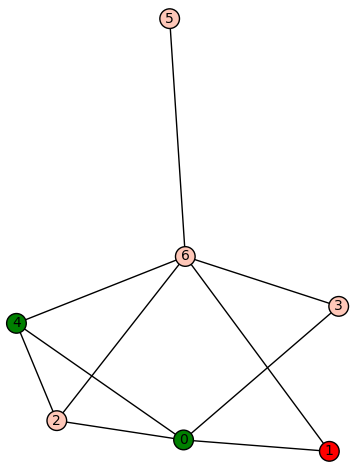
\includegraphics[width=6cm]{Images/Introduction/output_96_1.png}
\end{outImage}

\subsubsection{Some well-known graphs and graph families}

The famous Petersen graph.
\begin{sageCell}
    graphs.PetersenGraph()
\end{sageCell}
\begin{outImage}
    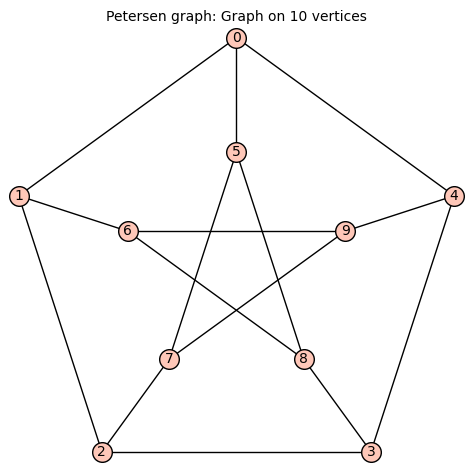
\includegraphics[width=8cm]{Images/Introduction/output_petersen.png}
\end{outImage}

Complete graphs $K_n$.
\begin{sageCell}
    graphs.CompleteGraph(7)
\end{sageCell}
\begin{outImage}
    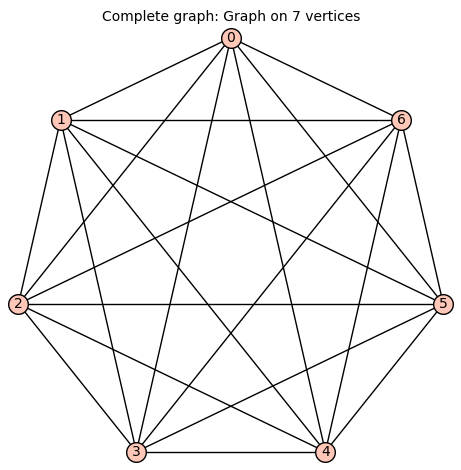
\includegraphics[width=8cm]{Images/Introduction/output_complete_7.png}
\end{outImage}

Cycle graphs $C_n$.
\begin{sageCell}
    graphs.CycleGraph(10)
\end{sageCell}
\begin{outImage}
    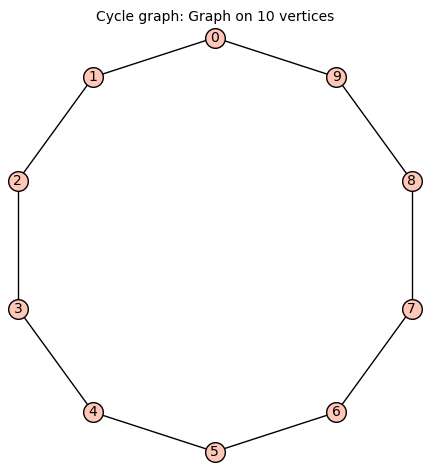
\includegraphics[width=8cm]{Images/Introduction/output_cycle_10.png}
\end{outImage}

Complete bipartite graphs $K_{n,m}$.
\begin{sageCell}
    graphs.CompleteBipartiteGraph(4, 10)
\end{sageCell}
\begin{outImage}
    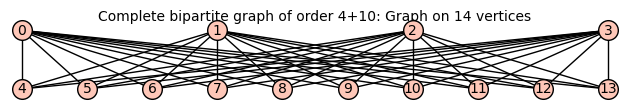
\includegraphics[width=0.8\linewidth]{Images/Introduction/output_complete_bipartite_4_10.png}
\end{outImage}

Grid graphs $G_{n,m}$.
\begin{sageCell}
    GG = graphs.GridGraph([4, 5])
    GG.plot()
\end{sageCell}
\begin{outImage}
    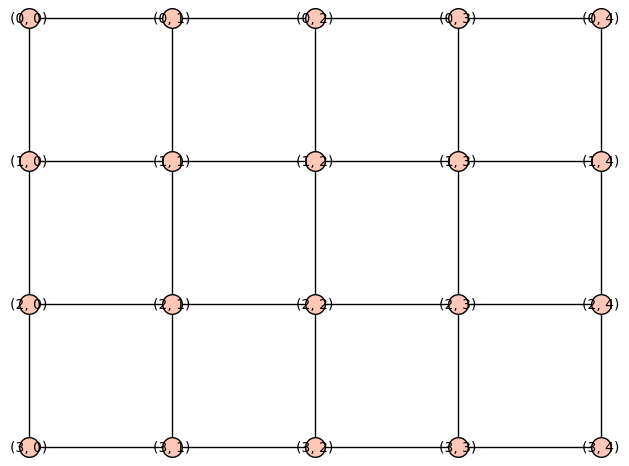
\includegraphics[width=0.8\linewidth]{Images/Introduction/output_grid_4_5.png}
\end{outImage}

\subsubsection{Randomly generated graphs}

Random graph on 10 nodes. Each edge is inserted independently with probability 0.3.
\begin{sageCell}
    graphs.RandomGNP(10, 0.3)
\end{sageCell}
\begin{outImage}
    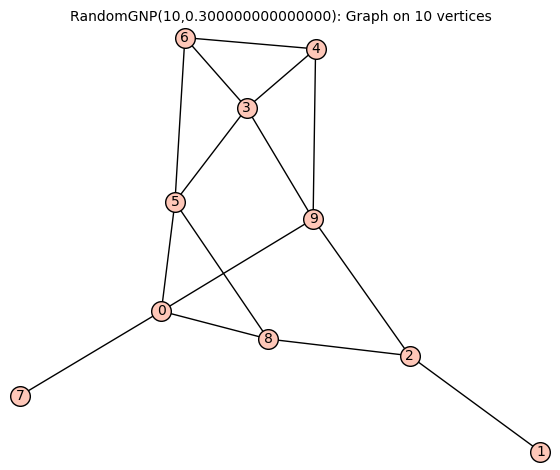
\includegraphics[width=0.8\linewidth]{Images/Introduction/output_random_10_03.png}
\end{outImage}

\subsubsection{Graph constructors}

From a list of edges.
\begin{sageCell}
    Graph([(1,2),(2,3),(3,1),(4,5)])
\end{sageCell}
\begin{outImage}
    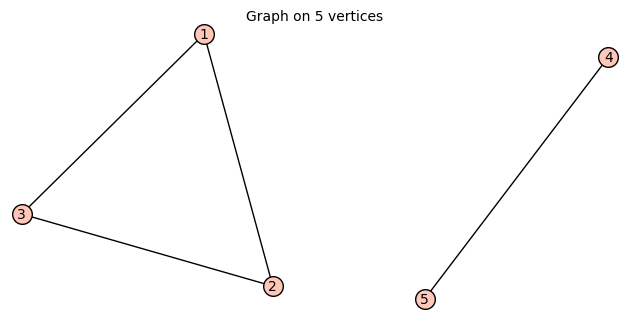
\includegraphics[width=10cm]{Images/Introduction/output_edge_list.png}
\end{outImage}

From an adjacency matrix.
\begin{sageCell}
    m = matrix([[int(i != j) for i in range(4)] for j in range(4)])
    m
\end{sageCell}
\begin{outCell}
    [0 1 1 1]
    [1 0 1 1]
    [1 1 0 1]
    [1 1 1 0]
\end{outCell}

\begin{sageCell}
    Graph(m)
\end{sageCell}
\begin{outImage}
    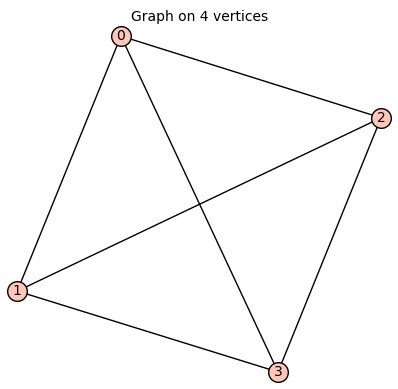
\includegraphics[width=6cm]{Images/Introduction/output_adjacency_matrix.png}
\end{outImage}

Graph to adjacency matrix.
\begin{sageCell}
    M = G.adjacency_matrix()
    m
\end{sageCell}
\begin{outCell}
    [0 1 1 1 1 0 0]
    [1 0 0 0 0 0 1]
    [1 0 0 0 1 0 1]
    [1 0 0 0 0 0 1]
    [1 0 1 0 0 0 1]
    [0 0 0 0 0 0 1]
    [0 1 1 1 1 1 0]
\end{outCell}

From/to graph6 format (compressed string representation of a graph).
\begin{sageCell}
    G = Graph('IheA@GUAo')
    G.plot()
\end{sageCell}
\begin{outImage}
    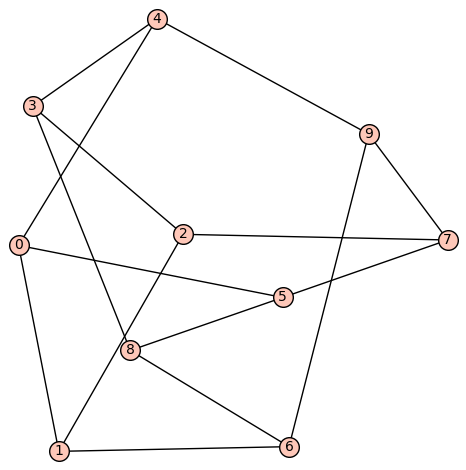
\includegraphics[width=6cm]{Images/Introduction/output_graph6.png}
\end{outImage}
\begin{sageCell}
    G.graph6_string()
\end{sageCell}
\begin{outCell}
    'IheA@GUAo'
\end{outCell}

Query a graph from local database
\url{http://doc.sagemath.org/html/en/reference/graphs/sage/graphs/graph_database.html}.
For example to get a list of all graphs on 7 vertices with diameter 5.
\begin{sageCell}
    Q = GraphQuery(display_cols=['graph6'], num_vertices=7, diameter=5)
    Q.show()
\end{sageCell}
\begin{outCell}
    Graph6
    --------------------
    F?`po
    F?gqg
    F@?]O
    F@OKg
    F@R@o
    FA_pW
    FEOhW
    FGC{o
    FIAHo
\end{outCell}

\subsection{Basic graph manipulation}

\begin{sageCell}
    G = Graph({0:[1,2,3], 4:[0,2], 6:[1,2,3,4,5]});
\end{sageCell}

\subsubsection{Access edges, verices, neighbors, etc.}

Access edges.
\begin{sageCell}
    G.edges(labels=False)
\end{sageCell}
\begin{outCell}
    [(0,1),(0,2),(0,3),(0,4),(1,6),(2,4),(2,6),(3,6),(4,6),(5,6)]
\end{outCell}
Note: Edges can have labels. To get a list of edges without labels, use \texttt{labels=False} option. Without this option we get
\begin{outCell}
    [(0,1,None),(0,2,None),(0,3,None),(0,4,None),(1,6,None),(2,4,None),
    (2,6,None),(3,6,None),(4,6,None),(5,6,None)]
\end{outCell}

To check if there is an edge between two vertices use
\begin{sageCell}
    G.has_edge(1,2)
\end{sageCell}
\begin{outCell}
    False
\end{outCell}

Access vertices.
\begin{sageCell}
    G.vertices()
\end{sageCell}
\begin{outCell}
    [0,1,2,3,4,5,6]
\end{outCell}

Access neighbors of a vertex.
\begin{sageCell}
    G.neighbors(0)
\end{sageCell}
\begin{outCell}
    [1,2,3,4]
\end{outCell}

Degree of a vertex is a number of its neighbors
\begin{sageCell}
    G.degree(0)
\end{sageCell}
\begin{outCell}
    4
\end{outCell}

To list degrees of all vertices use
\begin{sageCell}
    G.degree()
\end{sageCell}
\begin{outCell}
    [4,3,3,2,3,2,5]
\end{outCell}

Access number of vertices, edges
\begin{sageCell}
    [G.num_verts(),G.num_edges()]
\end{sageCell}
\begin{outCell}
    [7,10]
\end{outCell}

Vertices of a graph can be any hashable objects, not just integers. For example:
\begin{sageCell}
    X=Graph({'A':[1,2],'B':[(1,2),5,'A']})
    X.plot()
\end{sageCell}
\begin{outImage}
    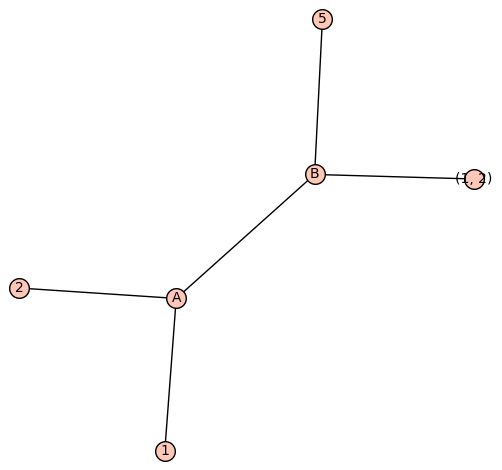
\includegraphics[width=8cm]{Images/Introduction/output_hashable.png}
\end{outImage}

\subsubsection{Add/remove vertices, edges}

Add a vertex.
\begin{sageCell}
    G.add_vertex('a')
\end{sageCell}

Method \verb|add_vertex| without arguments adds a single vertex with the smallest available label.
\begin{sageCell}
    newv = G.add_vertex()
    newv
\end{sageCell}
\begin{outCell}
    7
\end{outCell}

\begin{sageCell}
    G.vertices(sort=False)
\end{sageCell}
\begin{outCell}
    ['a',7,0,1,2,3,4,5,6]
\end{outCell}





\chapter{Depth-first search and Breadth-first search}

\section{Depth-first search (DFS)}

\subsection{Basic DFS implementation}

Write a Depth-first search (DFS) implementation using Sage Graph representation
\begin{itemize}
  \item Write a recursive implementation of the depth-first search.
  \item Add computation of discovery and finishing times to the implementation.
\end{itemize}
(See Handouts on Course Homepage for pseudocode)

\medskip
\begin{sageCell}
def DFS_recursive(G, r):
    """
    Perform DFS from root r. Result is a dictionary mapping a vertex v to
    its predecessor in DFS tree (root is mapped to None).
    """
    prev = {}
    prev[r] = None
    DFS_recursive_call(G, r, prev)
    return prev

def DFS_recursive_call(G, v, prev):
    for u in G.neighbors(v):
        if u not in prev:
            prev[u] = v
            DFS_recursive_call(G, u, prev)
\end{sageCell}

\subsubsection*{Examples}

\begin{sageCell}
   G = Graph({0:[1,2,3], 4:[0,2], 6:[1,2,3,4,5]})

   dfs_dict = DFS_recursive(G, 0)
   dfs_dict
\end{sageCell}
\begin{outCell}
   {0: None, 1: 0, 6: 1, 2: 6, 4: 2, 3: 6, 5: 6}
\end{outCell}

\begin{sageCell}
   G.plot(edge_colors={'red': [(u, v) for (u, v) in dfs_dict.items() if v != None]})
\end{sageCell}
\begin{outImage}
   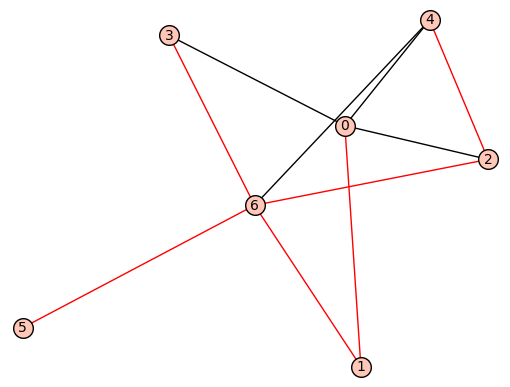
\includegraphics[width=0.5\textwidth]{Images/DFS/dfs_tree.png}
\end{outImage}

\begin{sageCell}
   H = graphs.Grid2dGraph(3, 3)
   DFS_recursive(H, (0, 0))
\end{sageCell}
\begin{outCell}
   {(0, 0): None,
    (0, 1): (0, 0),
    (0, 2): (0, 1),
    (1, 2): (0, 2),
    (1, 1): (1, 2),
    (1, 0): (1, 1),
    (2, 0): (1, 0),
    (2, 1): (2, 0),
    (2, 2): (2, 1)}
\end{outCell}

\subsection{DFS with start (discovery) time and end (finishing) time}

\begin{sageCell}
def DFS_with_times(G, r):
    """
    Perform DFS from root r. Result is a triple of three dictionaries:
    - dictionary mapping a vertex v to its predecessor in DFS tree
      (root is mapped to None).
    - dictionary mapping a vertex to its start time
    - dictionary mapping a vertex to its end time
    """
    global time
    time = 0
    prev = {}
    start = {}
    end = {}
    prev[r] = None
    DFS_with_times_call(G, r, prev, start, end)
    return (prev, start, end)

def DFS_with_times_call(G, v, prev, start, end):
    global time
    time += 1;
    start[v] = time;
    for u in G.neighbors(v):
        if u not in prev:
            prev[u] = v
            DFS_with_times_call(G, u, prev, start, end)
    time += 1;
    end[v] = time;
\end{sageCell}

\subsubsection*{Examples}

\begin{sageCell}
   G = Graph({0:[1,2,3], 4:[0,2], 6:[1,2,3,4,5]})
   (prev, disc, finish) = DFS_with_times(G, 0)
   (prev, disc, finish)
\end{sageCell}
\begin{outCell}
   ({0: None, 1: 0, 2: 6, 3: 6, 4: 2, 5: 6, 6: 1},
    {0: 1, 1: 2, 2: 4, 3: 8, 4: 5, 5: 10, 6: 3},
    {0: 14, 1: 13, 2: 7, 3: 9, 4: 6, 5: 11, 6: 12})
\end{outCell}

\begin{sageCell}
    G.relabel(dict([(v, (disc[v], finish[v])) for v in G.vertices()]))
    G.plot(edge_colors={'red': [((disc[u],finish[u]), (disc[v],finish[v]))
      for (u, v) in prev.items() if v != None]})
\end{sageCell}
\begin{outImage}
   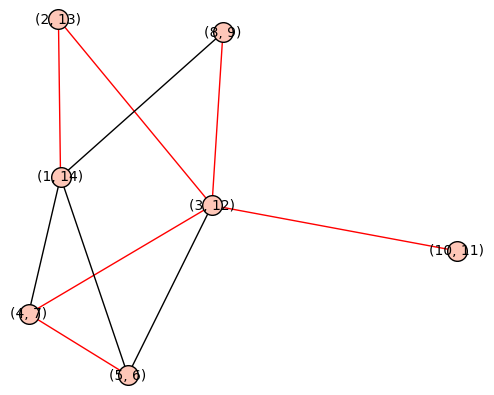
\includegraphics[width=0.6\textwidth]{Images/DFS/dfs_tree_with_times.png}
\end{outImage}

\section{Breadth-first search (BFS)}

Write a Breadth-first search (BFS) implementation using Sage Graph representation.

\medskip
\begin{sageCell}
import queue
def BFS(G, r):
    """
    Perform BFS from root r. Result is a dictionary mapping a vertex v
    to its predecessor in BFS tree (root is mapped to None).
    """
    prev = {}
    prev[r] = None
    q = queue.Queue()
    q.put(r)
    while not q.empty():
        v = q.get()
        for u in G.neighbors(v):
            if u not in prev:
                prev[u] = v
                q.put(u)
    return prev
\end{sageCell}

\subsubsection*{Example}

\begin{sageCell}
    BFS(H, (0, 0))
\end{sageCell}
\begin{outCell}
   {(0, 0): None,
    (0, 1): (0, 0),
    (1, 0): (0, 0),
    (0, 2): (0, 1),
    (1, 1): (0, 1),
    (2, 0): (1, 0),
    (1, 2): (0, 2),
    (2, 1): (1, 1),
    (2, 2): (1, 2)}
\end{outCell}

\section{Topological sorting}

\begin{itemize}
\item Use DFS with discovery and finishing times to implement topological sorting of a DAG (directed acyclic) graph
\item Help professor Bumstead to dress himself in the correct order. Order of putting his garments is given by the digraph below
\end{itemize}

\begin{sageCell}
    T = DiGraph({'undershorts': ['shoes','pants'],'pants':['shoes','belt'],'belt':['jacket'],'shirt':['belt','tie'],'tie':['jacket'],'socks':['shoes'],'watch':[]})
\end{sageCell}

\begin{sageCell}
def DFS_DiGraph(G):
    """
    Implement (recursive) DFS on a digraph to create a
    "forest of DFS trees"

    Use G.neighbors_out(v) to get "out" neighbors of vertex v
    """
    global time
    time = 0
    prev = {}
    start = {}
    end = {}
    for v in G.vertices(sort=False):
        if v not in prev:
            prev[v] = None
            DFS_DiGraph_call(G, v, prev, start, end)
    return (prev, start, end)

def DFS_DiGraph_call(G, v, prev, start, end):
    global time
    time += 1;
    start[v] = time;
    for u in G.neighbor_out_iterator(v):
        if u not in prev:
            prev[u] = v
            DFS_DiGraph_call(G, u, prev, start, end)
    time += 1
    end[v] = time
\end{sageCell}

\begin{sageCell}
    DFS_DiGraph(T)
\end{sageCell}
\begin{outCell}
    ({'belt': None,
      'jacket': 'belt',
      'tie': None,
      'watch': None,
      'shoes': None,
      'socks': None,
      'pants': None,
      'undershorts': None,
      'shirt': None},
     {'belt': 1,
      'jacket': 2,
      'tie': 5,
      'watch': 7,
      'shoes': 9,
      'socks': 11,
      'pants': 13,
      'undershorts': 15,
      'shirt': 17},
     {'jacket': 3,
      'belt': 4,
      'tie': 6,
      'watch': 8,
      'shoes': 10,
      'socks': 12,
      'pants': 14,
      'undershorts': 16,
      'shirt': 18})
\end{outCell}

\begin{sageCell}
def topological_sort(G):
    """
    Performs topological sort on a DAG (directed acyclic graph) G
    (calculate finishing times and sort vertices by them in
    descending order)
    """
    (_, _, finish) = DFS_DiGraph(T)
    return sorted(finish.items(), key=lambda x: -x[1])
\end{sageCell}

\begin{sageCell}
    topological_sort(T)
\end{sageCell}
\begin{outCell}
    [('shirt', 18),
     ('undershorts', 16),
     ('pants', 14),
     ('socks', 12),
     ('shoes', 10),
     ('watch', 8),
     ('tie', 6),
     ('belt', 4),
     ('jacket', 3)]
\end{outCell}


\chapter{Low value and 2-connected components}

\section{Low value}

For a vertex $v$, $\mathrm{low}(v)$ is the smallest discovery time, $\mathrm{disc}(x)$, over all vertices which can be reached from $v$ using tree edges (away from root) -- red edges -- and at most one back edge -- black edge.

In the example below labels of vertices are (vertex name, discovery time, low value) and arrows indicate parent of a vertex (prev).

\begin{center}
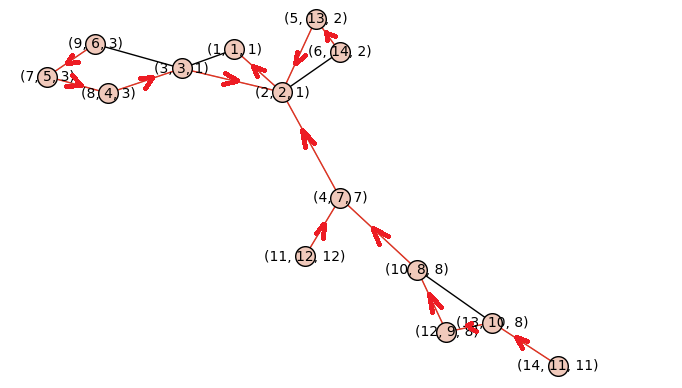
\includegraphics[width=0.9\textwidth]{Images/Low/low.png}
\end{center}

$\mathrm{low}(2)$ is $1$ since we can reach the root (with discovery time $1$) using red edge $(2, 3)$ and black edge $(3, 1)$.

$\mathrm{low}(8)$ is $3$ since the vertex with the smallest discovery time we can reach in the prescribed way is $3$: edges are $(8, 7), (7, 9), (9, 3)$ and $3$ has discovery time $3$.

$\mathrm{low}(10)$ is $8$ (its discovery time) since we can not reach any vertex with smaller discovery time using the tree edges "below" $10$.

\medskip
Use a recursive implementation of the depth-first search given in the previous chapter to compute the low value of each vertex in a graph.

\medskip
\begin{sageCell}
def DFS_low(G, r):
    """
    Calculate DFS with root r, discovery time, low values.
    """
    global time
    time = 0
    prev = {}
    disc = {}
    low = {}
    prev[r] = None
    DFS_low_call(G, r, prev, disc, low)
    return (prev, disc, low)

def DFS_low_call(G, v, prev, disc, low):
    global time
    time += 1;
    disc[v] = time;
    low[v] = time;
    for u in G.neighbors(v):
        if u not in prev:
            prev[u] = v
            DFS_low_call(G, u, prev, disc, low)
    for u in G.neighbors(v):
        if prev[u] == v:
            # edge (vertex) in "subtree"
            low[v] = min(low[v], low[u])
        elif u != prev[v]:
            # "back edge" and not a tree edge
            low[v] = min(low[v], disc[u])
\end{sageCell}

\subsubsection*{Example}

\begin{sageCell}
    G = Graph({1:[2,3], 2:[3,4,5,6], 3:[8,9], 4:[10,11], 5:[6], 7:[8,9],
    10:[12,13], 12:[13], 13:[14]})
    (prev, disc, low) = DFS_low(G, 1)
    low
\end{sageCell}
\begin{outCell}
    {1: 1,
     2: 1,
     3: 1,
     8: 3,
     7: 3,
     9: 3,
     4: 7,
     10: 8,
     12: 8,
     13: 8,
     14: 11,
     11: 12,
     5: 2,
     6: 2}
\end{outCell}

Relabel vertices with triples (vertex label, discovery time, low value) and color tree edges red

\begin{sageCell}
    G1 = G.relabel(dict([(v, (v, disc[v], low[v])) for
        v in G.vertices(sort=False)]), inplace=False)
    G1.plot(edge_colors={'red': [((u, disc[u], low[u]), (v, disc[v],
        low[v])) for (u, v) in prev.items() if v != None]})
\end{sageCell}
\begin{outImage}
    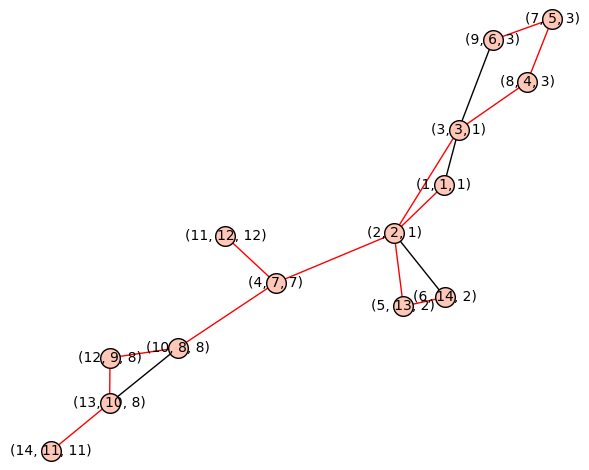
\includegraphics[width=0.9\textwidth]{Images/Low/output_low.png}
\end{outImage}

\section{Cutvertices}

We can get cutvertices using the following Theorem:

\begin{theorem}
Let $G$ be connected, undirected, simple, let $r$ be the root of its DFS tree $T$:
\begin{itemize}
\item $r$ is a cutvertex if it is incident with at least $2$ tree edges
\item nonroot vertex $v$ is a cutvertex if $v$ has a son $y$ so that $\mathrm{low}(y) \geq \mathrm{disc}(v)$
\end{itemize}
\end{theorem}

In the example above, cutvertices are $2, 3, 4, 10, 13$. For example, $10$ is a cutvertex, since its son in the tree has low value $8$ which is $\geq$ than discovery time of $10$, which is $8$.

Also, $4$ is a cutvertex since its sons ($11$ and $10$) have low values $\geq 7$
($7 = \mathrm{disc}(4)$).

The root $1$ is not a cutvertex since it is incident with only one tree edge.

\medskip
\begin{sageCell}
def cutvertices(G):
    """
    Retuns an array of cutvertices of a connected graph G.
    """
    root = G.vertices(sort=False)[0]     # assume G is connected
    (prev, start, low) = DFS_low(G, root)
    result = []
    rootn = 0
    for v in G.vertices(sort=False):
        for u in G.neighbors(v):
            if v != root:
                if v == prev[u] and low[u] >= start[v]:
                    result.append(v)
                    break
            elif v == prev[u]:
                rootn += 1
    if rootn >= 2:
        result.append(root)
    return result
\end{sageCell}

\subsubsection*{Example}

\begin{sageCell}
    cutvertices(G)
\end{sageCell}
\begin{outCell}
    [2, 3, 4, 13, 10]
\end{outCell}

\begin{sageCell}
    plot(G, vertex_colors={'red': cutvertices(G)})
\end{sageCell}
\begin{outImage}
    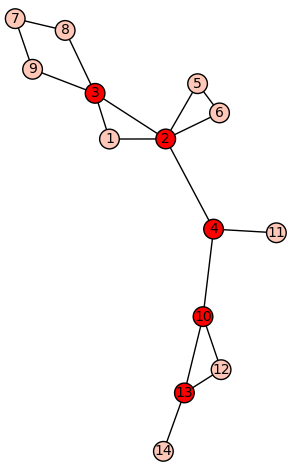
\includegraphics[width=0.45\textwidth]{Images/Low/output_cutvertices.png}
\end{outImage}

\section{2-connected components}

Write a function partition(G) which partitions edges of G into blocks (2-connected components).

Output should be a dictionary which maps an edge of the graph into a number which represents a block. In the example above, vertices $1, 2, 3$ (edges $(1,2), (1,3), (2,3)$) create a block. Therefore the resulting dictionary should map the pairs $(1,2), (1,3), (2,3)$ into the same number, say $1$.

\medskip
\begin{sageCell}
def partition(G):
    """"
    Partitions of edges of a connected graph G into blocks.
    Returns a dictionary mapping each edge to the block (number) it belongs to.
    """
    global blocknum
    root = G.vertices(sort=False)[0]     # assume G is connected
    (prev, start, low) = DFS_low(G, root)
    blocknum = 0
    blocks = {}
    partition_call(G, root, prev, start, low, blocks, 0)
    return blocks

def partition_call(G, v, prev, start, low, blocks, blockn):
    global blocknum
    for u in G.neighbors(v):
        if v == prev[u]: # forward tree edge
            if low[u] >= start[v]: # cut vertex, start a new block
                blocknum += 1
                blocks[(v, u)] = blocknum
                partition_call(G, u, prev, start, low, blocks, blocknum)
            else: # stay in the same block
                blocks[(v, u)] = blockn
                partition_call(G, u, prev, start, low, blocks, blockn)
        elif start[u] < start[v] and u != prev[v]: # back edge not in tree
            blocks[(u, v)] = blockn
\end{sageCell}

\subsubsection*{Example}

\begin{sageCell}
    partition(G)
\end{sageCell}
\begin{outCell}
    {(10, 4): 1,
     (4, 2): 2,
     (2, 1): 3,
     (1, 3): 3,
     (2, 3): 3,
     (3, 8): 4,
     (8, 7): 4,
     (7, 9): 4,
     (3, 9): 4,
     (2, 5): 5,
     (5, 6): 5,
     (2, 6): 5,
     (4, 11): 6,
     (10, 12): 7,
     (12, 13): 7,
     (10, 13): 7,
     (13, 14): 8}
\end{outCell}

\begin{sageCell}
import random
def edge_colors(part):
    blocks = set(part.values())
    colors = [(random.random(), random.random(), random.random()) for b in blocks]
    colorblocks = [[edge for edge in part.keys() if part[edge] == b] for b in blocks]
    return dict(zip(colors, colorblocks))
\end{sageCell}
\begin{sageCell}
    G.plot(edge_colors=edge_colors(partition(G)))
\end{sageCell}
\begin{outImage}
    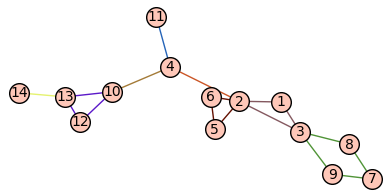
\includegraphics[width=0.6\textwidth]{Images/Low/output_partition.png}
\end{outImage}


\chapter{Shortest Hamiltonian cycle (Travelling salesman problem)}

The travelling salesman problem (TSP) asks the following question: "Given a list of cities and the distances between each pair of cities, what is the shortest possible route that visits each city exactly once and returns to the origin city?"

We will assume that there are roads (edges) between all cities (complete graph) and that the distances are Euclidean distances (Euclidean TSP).

We will write an approximation algorithm for TSP, which will be based on the minimum spanning tree (MST) algorithm.

\section{Approximation}

Implement the following 2-approximation algorithm (that means that the length of our solution will be better than 2 times the length of an optimal solution).
\begin{enumerate}
    \item Find minimal spanning tree of our graph (use built-in Sage function \verb`min_spanning_tree`).
    \item Run DFS on this tree.
    \item Take vertices in the order of increasing (DFS) start time.
\end{enumerate}

\medskip
\begin{sageCell}
def TSP_approximation(G):
    """
    Returns Hamiltonian cycle (travelling salesman circuit) using a 2-approximation algorithm.
    """
    mst = G.min_spanning_tree(by_weight=True)
    T = Graph(mst) # graph (tree) from edges

    # DFS with times
    r = T.vertices(sort=False)[0]
    _, start, _ = DFS_with_times(T, r)
    sort_start = sorted(list(start.items()), key=lambda p: p[1])
    cycle = []
    length = 0
    sort_start.append(sort_start[0])
    for i in range(1, len(sort_start)):
        u = sort_start[i - 1][0]
        v = sort_start[i][0]
        cycle.append((u, v))
        length += G.edge_label(u, v)
    return cycle, length
\end{sageCell}

\subsubsection*{Example}

Create the test example, a complete graph with 10 vertices with given vertex coordinates.

\medskip
\begin{sageCell}
def distance(a, b):
    """
    Return Euclidean distance between a = (ax, ay) and b = (bx, by)
    """
    ax, ay = a
    bx, by = b
    return math.sqrt((bx - ax)**2 + (by - ay)**2)

def set_euclidean_distances(G):
    """
    Set Euclidean distances as edge weights (labels)
    """
    pos = G.get_pos()
    for (u, v) in G.edges(sort=False, labels=False):
        G.set_edge_label(u, v, distance(pos[u], pos[v]))

H = graphs.CompleteGraph(10)
H.set_pos({0: [8, 1], 1: [0, 8], 5: [1, 0], 2: [5, 3], 3: [1.5, 7], 4: [2, 4],
  6: [6, 2], 7: [3, 1], 8: [2, 2], 9: [3, 3]})
set_euclidean_distances(H)
\end{sageCell}

\begin{sageCell}
    cycle, length = TSP_approximation(H)
\end{sageCell}
\begin{sageCell}
    cycle, length
\end{sageCell}
\begin{outCell}
   ([(0, 6),
     (6, 2),
     (2, 9),
     (9, 4),
     (4, 3),
     (3, 1),
     (1, 8),
     (8, 5),
     (5, 7),
     (7, 0)], 27.70534328046342)
\end{outCell}

Compare with the optimal solution, computed using the built-in Sage function\\ \verb`traveling_salesman_problem`.

\medskip
\begin{sageCell}
    def cycle_length(cycle, G):
        length = 0
        for u, v in cycle:
            length += G.edge_label(u, v)
        return length

    opt_cycle = H.traveling_salesman_problem(use_edge_labels=True)
    opt_length = cycle_length(opt_cycle.edges(sort=False, labels=False),
      opt_cycle)
    opt_length
\end{sageCell}
\begin{outCell}
    27.540829118717557
\end{outCell}

\section{Iterative improvement}

\subsection{2-changes on intersecting segments}

Improve a solution iteratively using 2-changes on \emph{intersecting} segments.

A \emph{2-change} is a transformation of a cycle by removing two non-consecutive edges and adding two other edges such that the resulting graph is still a cycle.

\medskip
\begin{sageCell}
def iterate_2_changes_intersecting(cycle, G, n=1000):
    """
    Iterate by eliminating intersections by 2-changes. Make at most n iterations
    """
    for k in range(n):
        inter = find_intersection(cycle, G)
        if inter == None:
            return cycle
        i, j = inter
        cycle = perform_2_change(cycle, i, j)
    return cycle
\end{sageCell}
(See the code for \verb`find_intersection` and \verb`perform_2_change` at the end of this chapter.)

\subsubsection*{Example}

\begin{sageCell}
    cycle = [(0, 1), (1, 2), (2, 3), (3, 4), (4, 5), (5, 6), (6, 7), (7, 8), (8, 9),
      (9, 0)]
    new_cycle = iterate_2_changes_intersecting(cycle, H, 10)
    (cycle_length(new_cycle, H), cycle_length(cycle, H))
\end{sageCell}
\begin{outCell}
    (30.367268577721603, 46.94180782091779)
\end{outCell}

\subsection{2-changes on random edges}

Improve a solution iteratively using 2-changes on \emph{random}
non-adjacent cycle edges.

\medskip
\begin{sageCell}
def iterate_2_changes(cycle, G, n):
    min_length = cycle_length(cycle, G)
    min_cycle = cycle
    for k in range(n):
        i = randint(0, len(min_cycle) - 1)
        add = randint(2, len(min_cycle) - 2)
        j = (i + add) % len(min_cycle)
        new_cycle = perform_2_change(min_cycle, i, j)
        new_length = cycle_length(new_cycle, G)
        if new_length < min_length:
            min_length = new_length
            min_cycle = new_cycle
    return min_cycle
\end{sageCell}

\subsubsection*{Example}

\begin{sageCell}
    new_cycle = iterate_2_changes(cycle, H, 50000)
    (cycle_length(new_cycle, H), cycle_length(cycle, H))
\end{sageCell}
\begin{outCell}
    (27.669330960262805, 46.94180782091779)
\end{outCell}
\begin{sageCell}
    (cycle_length(new_cycle, H), opt_length)
\end{sageCell}
\begin{outCell}
    (27.669330960262805, 27.540829118717557)
\end{outCell}


\subsection{Code of auxiliary functions}

\begin{sageCell}
def perform_2_change(cycle, i, j):
    """
    Perform a 2-change on a (hamiltonian) cycle for edges with
    (non-consecutive) indices i and j. Cycle is a list of edges
    """
    if i > j:
        i, j = j, i
    e1 = cycle[i]
    e2 = cycle[j]
    v1, u1 = e1
    v2, u2 = e2
    result = []
    revert = False
    for k in range(i):
        result.append(cycle[k])
    result.append((v1, v2))
    for k in reversed(range(i + 1, j)):
        result.append(tuple(reversed(cycle[k])))
    result.append((u1, u2))
    for k in range(j + 1, len(cycle)):
        result.append(cycle[k])
    return result
\end{sageCell}

Intersection of two segments.
\begin{sageCell}
def find_intersection(cycle, G):
    """
    Find indices of two non-consecutive cycle edges which intersect and None if there are none
    """
    pos = G.get_pos()
    for i in range(len(cycle)):
        ei = cycle[i]
        l = len(cycle) if i > 0 else len(cycle) - 1
        for j in range(i + 2, l):
            ej = cycle[j]
            if do_intersect(pos[ei[0]], pos[ei[1]], pos[ej[0]], pos[ej[1]]):
                return (i, j)
    return None

def on_segment(p, q, r):
    if ((q[0] <= max(p[0], r[0])) and (q[0] >= min(p[0], r[0])) and
        (q[1] <= max(p[1], r[1])) and (q[1] >= min(p[1], r[1]))):
        return True
    return False

def orientation(p, q, r):
    val = (float(q[1] - p[1]) * (r[0] - q[0])) - (float(q[0] - p[0]) * (r[1] - q[1]))
    if (val > 0):
        return 1
    elif (val < 0):
        return 2
    else:
        return 0

# Check if two segments intersect
# https://www.geeksforgeeks.org/check-if-two-given-line-segments-intersect/
def do_intersect(p1, q1, p2, q2):
    o1 = orientation(p1, q1, p2)
    o2 = orientation(p1, q1, q2)
    o3 = orientation(p2, q2, p1)
    o4 = orientation(p2, q2, q1)

    if ((o1 != o2) and (o3 != o4)):
        return True
    if ((o1 == 0) and on_segment(p1, p2, q1)):
        return True
    if ((o2 == 0) and on_segment(p1, q2, q1)):
        return True
    if ((o3 == 0) and on_segment(p2, p1, q2)):
        return True
    if ((o4 == 0) and on_segment(p2, q1, q2)):
        return True
    return False
\end{sageCell}





\chapter{Graph drawing}

In this chapter, we will write \emph{iterative} methods for drawing graphs. General idea is to:
\begin{enumerate}
\item Start with a random drawing of a graph
\item Iteratively improve the drawing
\end{enumerate}

\section{Method 1: Mass center}

Write the following functions:
\begin{enumerate}
\item \verb|move_vertex_c(G, v, pos)|\\
    Where $G$ is graph, $v$ is a vertex in $G$ and $\mathrm{pos}$ is a dictionary of positions for each vertex. It should move position of $v$ to the mass center of its neighbors, i.e., $\mathrm{pos}(v) = 1/|N(v)| \sum_{u \in N(v)} \mathrm{pos}(u)$.
\item \verb|draw_graph_c(G, F, iters)|\\
    Where $G$ is graph, $F$ is a list of fixed vertices, $\mathrm{iters}$ is a number of iterations. Function should
    \begin{enumerate}
        \item Draw positions of vertices of $F$ on a circle (with radius 1, i.e., set positions of $F$ to vertices of a regular polygon).
        \item Other vertices, $V(G)\setminus F$, set to random positions in square $[-0.5, 0.5] \times [-0.5, 0.5]$.
        \item Use function \verb|move_vertex_c| to change the position of each vertex $V(G)\setminus F$.
        \item Repeat Step 3 $\mathrm{iters}$ times.
    \end{enumerate}
\end{enumerate}

\medskip
\begin{sageCell}
def move_vertex_c(G, v, pos):
    """
    Move vertex v to the mass center of its neighbors.
    """
    sx = 0
    sy = 0
    N = 0
    for u in G.neighbors(v):
        x,y = pos[u]
        sx += x
        sy += y
        N += 1
    if N > 0:
        pos[v] = (sx/N, sy/N)
\end{sageCell}
\begin{sageCell}
def draw_graph_c(G, F, iters):
    """
    Draw graph G with fixed vertices F using mass center method.
    """
    pos = {}
    for i in range(len(F)):
        pos[F[i]] = (cos(2*i*math.pi/len(F)), sin(2*i*math.pi/len(F)))
    vert = [v for v in G.vertices(sort=False) if v not in F]
    for v in vert:
        pos[v] = (random() - 0.5, random() - 0.5)
    for i in range(iters):
        for v in vert:
            move_vertex_c(G, v, pos)
    G.set_pos(pos)
    return G.plot(vertex_labels = False, vertex_size = 10)
\end{sageCell}
Example:
\begin{sageCell}
def find_cycle(G0):
    """
    An ad-hoc function to find some cycle in a graph, provided that G is 2-connected
    """
    G = G0.copy()
    e = G.edges(sort=False)[0]
    G.delete_edge(e)
    return G.shortest_path(e[0], e[1])
\end{sageCell}
\begin{sageCell}
    G = graphs.BuckyBall()
    draw_graph_c(G, find_cycle(G), 5)
\end{sageCell}

\begin{outImage}
    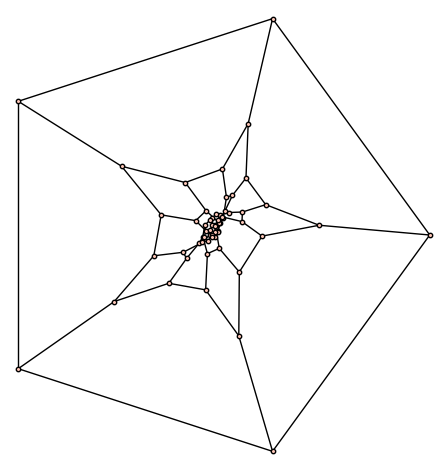
\includegraphics[width=0.5\textwidth]{Images/Drawing/bucky_ball_mass_5.png}
\end{outImage}

\begin{sageCell}
    G = graphs.BuckyBall()
    draw_graph_c(G, find_cycle(G), 100)
\end{sageCell}
\begin{outImage}
    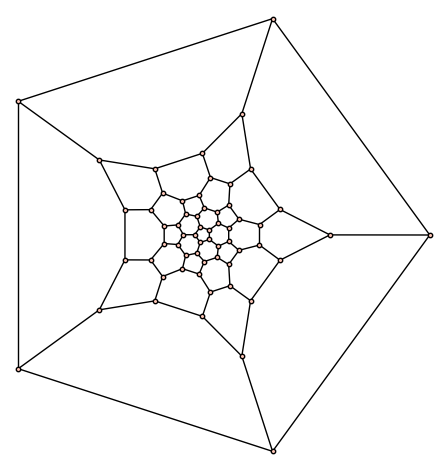
\includegraphics[width=0.5\textwidth]{Images/Drawing/bucky_ball_mass_100.png}
\end{outImage}

\section{Method 2: Move vertices using force}

Write the following functions:
\begin{enumerate}
\item \verb|move_vertex_f(G, v, pos, k)|\\
    Where $G$ is graph, $v$ is a vertex in $G$, $\mathrm{pos}$ is a dictionary of positions for each vertex and $k$ is a constant.
    Similar to \verb|move_vertex_c|, just use "forces" to move vertex $v$. Each edge $vu$ ($u$ is a neighbor of $v$) acts like a "spring" and acts with force $\vec{F} = k\: \vec{\delta}$ where $\vec{\delta} = \vec{u} - \vec{v}$ (Hooke's law) and $k$ is characteristic of the spring (razteznostni koeficient in Slovene). That is: $\mathrm{pos}(v) = \mathrm{pos}(v) + \sum_{u \in N(v)} k (\mathrm{pos}(u) - \mathrm{pos}(v))$.
\item \verb|draw_graph_f(G, F, k, iters)|\\
    which acts in the same way as \verb|draw_graph_c|, but it uses the function \verb|move_vertex_f| instead of \verb|move_vertex_c|.
\end{enumerate}

\medskip
\begin{sageCell}
def move_vertex_f(G, v, pos, k):
    """
    Move vertex v using force method.
    """
    vx, vy = pos[v]
    fx, fy = pos[v]
    for u in G.neighbors(v):
        x,y = pos[u]
        dx = x - vx
        dy = y - vy
        fx += dx * k
        fy += dy * k
    pos[v] = (fx, fy)


def draw_graph_f(G, F, k, iters):
    pos = {}
    for i in range(len(F)):
        pos[F[i]] = (cos(2*i*math.pi/len(F)), sin(2*i*math.pi/len(F)))
    vert = [v for v in G.vertices(sort=False) if v not in F]
    for v in vert:
        pos[v] = (random() - 0.5, random() - 0.5)
    for i in range(iters):
        for v in vert:
            move_vertex_f(G, v, pos, k)
    G.set_pos(pos)
    return G.plot(vertex_labels = False, vertex_size = 10)
\end{sageCell}
\begin{sageCell}
    G = graphs.BuckyBall()
    draw_graph_f(G, find_cycle(G), 0.1, 100)
\end{sageCell}
\begin{outImage}
    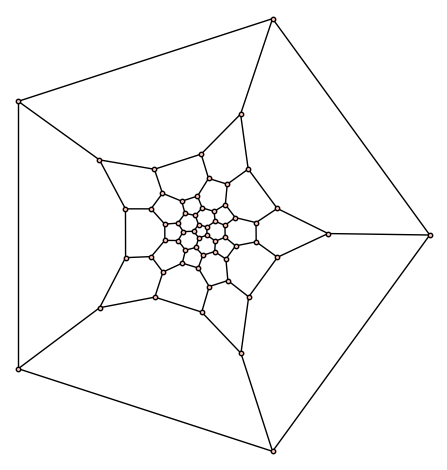
\includegraphics[width=0.5\textwidth]{Images/Drawing/bucky_ball_force_100.png}
\end{outImage}

\section{Method 3: Spring embedder}

For both methods above we required a cycle to be selected before fixing its coordinates. But this is not "practical". Can we do without this?
Without fixing some vertices, and using only the (attractive) force method, the vertices of the graph will eventually move to a single point. So we need to add \emph{repulsive} forces.

\begin{enumerate}
    \item \verb|move_vertex_se(G, v, pos, k, e)|\\
    Similar to \verb|move_vertex_f|, each edge $vu$ acts like a "spring" and acts with force $
    \vec{F} = k\: \vec{\delta}$ where $\vec{\delta} = \vec{u} - \vec{v}$. Additionally: vertices also act in a repulsive way with force $\vec{R} = -e\: \vec{\delta}/|\vec{\delta}|^2$ for all $u \neq v$. With the repulsive force we do not allow two vertices to be too close, since the force is inversely proportional to the square of the distance between them!
    \item \verb|draw_graph_se(G, k, e, iters)|\\
    Similar to \verb|draw_graph_f|, just use \verb|move_vertex_se| instead of \verb|move_vertex_f|. Note that there are no fixed vertices. Initially, for each vertex, choose a random position in the square $[-0.5, 0.5] \times [-0.5, 0.5]$.
\end{enumerate}

\medskip
\begin{sageCell}
    def move_vertex_se(G, v, pos, k, e):
    vx, vy = pos[v]
    fx, fy = pos[v]
    for u in G.neighbors(v):
        x,y = pos[u]
        dx = x - vx
        dy = y - vy
        fx += dx * k
        fy += dy * k
    for u in G.vertices(sort=False):
        if v == u:
            continue
        x, y = pos[u]
        dx = x - vx
        dy = y - vy
        r2 = dx*dx + dy*dy
        fx += -e*dx/r2
        fy += -e*dy/r2
    pos[v] = (fx, fy)


def draw_graph_se(G, k, e, iters):
    pos = {}
    for v in G.vertices(sort=False):
        pos[v] = (random() - 0.5, random() - 0.5)
    for i in range(iters):
        for v in G.vertices(sort=False):
            move_vertex_se(G, v, pos, k, e)
    G.set_pos(pos)
    return G.plot(vertex_labels = False, vertex_size = 10)
\end{sageCell}

For the graphs below, try to find $k$ and $e$ such that the result will be "nice".

\begin{sageCell}
    G = graphs.BuckyBall()
    draw_graph_se(G, ?, ?, 100)
\end{sageCell}
\begin{outImage}
    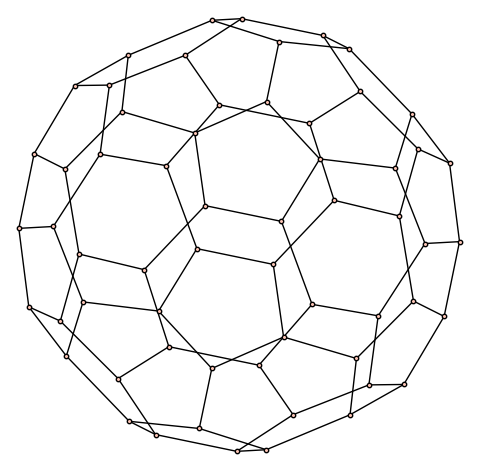
\includegraphics[width=0.5\textwidth]{Images/Drawing/bucky_ball_se_100.png}
\end{outImage}

More examples
\begin{sageCell}
    draw_graph_se(graphs.Grid2dGraph(10, 10), ?, ?, 100)

    draw_graph_se(graphs.CycleGraph(10), ?, ?, 100)

    C10 = graphs.CycleGraph(10)
    C4 = graphs.CycleGraph(4)
    draw_graph_se(C10.cartesian_product(C4), ?, ?, 100)

    draw_graph_se(graphs.RandomTree(100), ?, ?, 100)

    draw_graph_se(Graph('ShCHGD@?K?_@?@?C_GGG@??cG?G?GK_?C'), ?, ?, 100)
\end{sageCell}


\chapter{3-coloring planar graphs without short cycles}

\section{Introduction}

The chromatic number $\chi(G)$ of a graph $G$ is the smallest number of colors that suffice to color the vertices of $G$ such that no two adjacent vertices have the same color.

The well known Four Color Theorem states that for every planar graph is $\chi{G} \leq 4$.

It is NP-hard to decide if $\chi(G) \leq 3$ if $G$ is planar, but:
\begin{theorem}
Let $G$ be a planar graph without cycles of lengths $4, \ldots, 11$. Then $\chi(G) \leq 3$.
\end{theorem}

\section{Discharging method}

Discharging method idea (see \href{http://webdocs.cs.ualberta.ca/~mreza/talks/IPM-math06.pdf}{"Discharging method, by M. Salavatipour} for more details).

\medskip
\noindent If the theorem is not true and $G$ is a smallest counterexample, then there is:
\begin{enumerate}
    \item no vertex of degree $\leq 2$ and
    \item no cutvertex.
\end{enumerate}
If we apply the following discharging method:
\begin{enumerate}
    \item assign a charge of $deg(v) - 6$ units to each vertex $v$ of $G$ and of $2 |f| - 6$ to each face $f$ of $G$ and
    \item the rule for discharging is: each non-triangle face sends 3/2 units to each of its vertices
\end{enumerate}
then we come to a contradiction with the initial total charge of $-12$ and the final charge $\geq 0$. Thus, there is either a vertex of degree $\leq 2$ or a cutvertex in such graphs.

This gives us an algorithm to color such graphs with 3 colors:
\begin{enumerate}
\item If we find a vertex of degree $\leq 2$ we can remove it, recursively color the rest of the graph and color the removed vertex with the color missing in its two neighbors.
\item If we find a cutvertex, we split the graph into two (or more) blocks, recursively color the blocks, make sure that the removed vertex gets the same color in all blocks and color the removed vertex with that color.
\end{enumerate}

\section{Exercises}

\begin{enumerate}
    \item Write a function \verb|initial_charge(G)| which returns dicitionary with initial charges of vertices and faces.
    \item Write a function \verb|discharge(G, c0)| which returns dictionary with charges after discharging was applied to the initial charges \verb|c0| (result of \verb|initial_charge(G)|).
    \item Write a function \verb|plot_charge(G, c)| which plots vertices with green color if they have non-negative charge and with red color if they are negatively charged (\verb|c| is result of the function \verb|plot_charge(G, c)|).
    \item Write a function \verb|three_color(G)| which implements the algorithm for three coloring of $G$ described above.
\end{enumerate}
You can use Sage built-in function \verb|blocks_and_cut_vertices| to find cutvertices and blocks.

\section{Solutions}

\begin{sageCell}
    def faces(G):
    """
    Return faces (as "tuples" of vertices) of a planar graph G.
    """
    G.is_planar(set_embedding=True)
    F = G.faces()
    F = [tuple(x for (x, y) in f) for f in F]
    return F

def initial_charge(G):
    """
    Return a dictionary of charges for each vertex and face
    """
    F = faces(G)
    c = {}
    for v in G.vertices():
        c[v] = G.degree(v) - 6
    for f in F:
        c[f] = 2 * len(f) - 6
    return c

def discharge(G, c0):
    """
    Return a dictionary of charges for each vertex and face after discharging initial charges c0
    """
    c = c0.copy()
    F = faces(G)
    for f in F:
        if len(f) > 3:
            for v in f:
                c[v] += 3/2
                c[f] -= 3/2
    return c

def plot_colored_charges(G, c):
    """
    Plot negatively charged vertices of G with red and non-negatively charged vertices of G with green;
    according to charges given by the dictionary c
    """
    v_pos = [v for v in G.vertices() if c[v] >= 0]
    v_neg = [v for v in G.vertices() if c[v] < 0]
    return G.plot(vertex_colors = {'green': v_pos, 'red': v_neg}, vertex_size=20, vertex_labels=False)
\end{sageCell}

\begin{sageCell}
    def three_color(G):
    '''
    Return 3 coloring of planar graph G without cycles of length 4, ..., 11.
    Coloring is represented as a dicitionary mapping a vertex to one of the colors 0, 1, 2.
    '''
    if G.num_verts() == 1:
        return {G.vertices()[0]: 0}

    G = G.copy()

    # find a cutvertex
    blocks, c_vertices = G.blocks_and_cut_vertices()
    if len(c_vertices) > 0:
        cutv = c_vertices[0]
        nbs = G.neighbors(cutv)
        result = dict()
        G.delete_vertex(cutv)
        for C in G.connected_components_subgraphs():
            # color subgraphs such that cutv has color 0
            c = three_color_cv(C, cutv, nbs)
            for v, color in c.items():
                result[v] = color
        return result

    # find a vertex of degree <= 2
    v = min(G.vertices(), key=lambda v: G.degree(v))
    if G.degree(v) <= 2:
        nbs = G.neighbors(v)
        G.delete_vertex(v)
        c = three_color(G)
        freec = list(set([0, 1, 2]) - set([c[u] for u in nbs]))
        c[v] = freec[0]
        return c
    raise Exception('No substructure')

# color G such that cutv has color 0
def three_color_cv(G, cutv, cutvnbs):
    gverts = set(G.vertices())
    G = G.copy()
    G.add_vertex(cutv)
    for u in cutvnbs:
        if u in gverts:
            G.add_edge(cutv, u)
    c = three_color(G)
    cvc = c[cutv] # color of cut vertex, we will change colors such that cvc will be 0
    if cvc == 0:  # ok, cut vertex has color 0
        return c
    cr = dict()
    # switch colors 0 and cvc
    for v, col in c.items():
        if col == cvc:  # color cvc -> color 0
            cr[v] = 0
        elif col == 0: # color 0 -> color cvc
            cr[v] = cvc
        else:
            cr[v] = col
    return cr
\end{sageCell}

\chapter{5-coloring of planar graphs}

Write the following recirsive algorithm for 5-coloring of planar graphs:

\medskip
\noindent Find a vertex $x$ of minimum degree.
\begin{enumerate}
    \item if the vertex $x$ is of degree 4 or less, remove it, color the smaller graph and extend the coloring to $x$,
    \item f the vertex $x$ is of degree 5 remove it, identify two non-adjacent neighbors $u$ and $v$ of $x$, color the smaller graph and extend the coloring to $x$. Note: if the neighbors of $x$ in the \textbf{embedding} are $x_0$, $x_1$, $x_2$, $x_3$, $x_4$ then either we take $u$ = $x_0$ and $v$ = $x_2$, if $x_0$ and $x_2$ are not adjacent, or $u$ = $x_1$ and $v$ = $x_3$, otherwise.
\end{enumerate}

\medskip
\noindent \textbf{Note:}
Use the following built-in Sage methods on graphs:
\begin{itemize}
\item \verb|G.is_planar(set_embedding=True, set_pos=True)| checks for planarity and, optionally, sets coordinates and combinatorial embedding (clockwise ordering of neighbors at each vertex)
\item  Subsequent call to the method \verb|G.faces()| returs the faces of the graph (as lists of edges) and a call to the method \verb|G.get_embedding()| returns the combinatorial embedding (mapping from vertices to lists of neighbors in clockwise order around the vertex).
\item  \verb|G.plot()| plots the graph with the given embedding and coordinates (if it is planar).
\end{itemize}

\medskip
Example:
\begin{sageCell}
    H = Graph({0:[1,2,3], 1:[4,5], 2:[6], 3:[4,6], 4:[7], 5:[7], 6:[7]})
    H.is_planar(set_embedding=True, set_pos=True)
\end{sageCell}
\begin{outCell}
    True
\end{outCell}

\begin{sageCell}
    H.plot()
\end{sageCell}
\begin{outImage}
   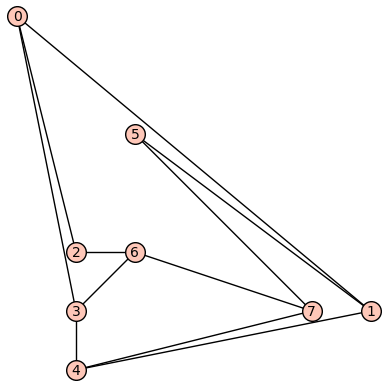
\includegraphics[width=0.6\textwidth]{Images/5-coloring/planar_graph.png}
\end{outImage}

\begin{sageCell}
    H.faces()
\end{sageCell}
\begin{outCell}
    [[(0, 1), (1, 4), (4, 3), (3, 0)],
     [(0, 2), (2, 6), (6, 7), (7, 5), (5, 1), (1, 0)],
     [(0, 3), (3, 6), (6, 2), (2, 0)],
     [(1, 5), (5, 7), (7, 4), (4, 1)],
     [(3, 4), (4, 7), (7, 6), (6, 3)]]
\end{outCell}

\begin{sageCell}
    H.get_embedding()
\end{sageCell}
\begin{outCell}
    {0: [1, 2, 3],
     1: [4, 5, 0],
     2: [0, 6],
     3: [0, 6, 4],
     4: [3, 7, 1],
     5: [1, 7],
     6: [2, 7, 3],
     7: [5, 4, 6]}
\end{outCell}

\section{Solution}

\begin{sageCell}
def color_planar_5(G):
    if not G.is_planar(set_embedding=True):
        raise Exception("Input is not a planar graph.")
    emb = G.get_embedding()

    return color_planar_5_rec(emb)
\end{sageCell}

\begin{sageCell}
def color_planar_5_rec(emb):
    # Graph has <= 5 vertices
    if len(emb) <= 5:
        vertices = emb.keys()
        col = dict(zip(vertices, [0, 1, 2, 3, 4]))
        return col

    # Find vertex with min degree
    x = min(emb, key = lambda v: len(emb[v]))

    if len(emb[x]) < 5:
        return color_planar_5_d4(emb, x)
    else:
        return color_planar_5_d5(emb, x)

def color_planar_5_d4(emb, x):

    # remove x from the graph
    Nx = emb[x]
    for w in Nx:
        emb[w].remove(x)
    del emb[x]

    # color the rest
    col = color_planar_5_rec(emb)

    # extend to x
    used = [col[w] for w in Nx]
    free = [c for c in [0, 1, 2, 3, 4] if c not in used]
    col[x] = free[0]

    return col

def color_planar_5_d5(emb, x):

    # choose u,v to identify
    Nx = emb[x]
    if Nx[0] in emb[Nx[2]]:
        u,v = Nx[1], Nx[3]
    else:
        u,v = Nx[0], Nx[2]

    # u and v have a common neighbor x,
    # for other common neighbors w we remove
    # the edge wu (no double edges!)
    for w in emb[v]:
        if w != x and w in emb[u]:
            emb[u].remove(w)
            emb[w].remove(u)

    # identify u and v
    ux = emb[u].index(x)
    vx = emb[v].index(x)
    emb[u] = emb[u][:ux] + emb[v][vx + 1:] + emb[v][:vx] + emb[u][ux + 1:]
    for w in emb[v]:
        wv = emb[w].index(v)
        emb[w][wv] = u
    del emb[v]

    # remove the vertex x
    for w in Nx:
        if w != u and w != v:
            emb[w].remove(x)
    del emb[x]

    # color the rest
    col = color_planar_5_rec(emb)

    # extend the coloring
    used = [col[w] for w in Nx if w in col]
    free = [c for c in [0, 1, 2, 3, 4] if c not in used]
    col[v] = col[u]
    col[x] = free[0]

    return col
\end{sageCell}




\chapter{List coloring of planar triangulations}

According to Thomassen's theorem every planar graph is 5-choosable. The algorithm for list coloring planar graphs is described in Lecture Notes available at \url{(http://matematika.fri.uni-lj.si/dm/discrete_mathematics.pdf}, Section 6.3.

\section{implementation}

Note: We can implement the algorithm without altering the input graph but we will, however, alter lists in the lists (we will remove colors from them).

\begin{sageCell}
def list_coloring(G, L):
    """
    Colors a planar triangulation `G` using colors in color map `L`; that is `L` maps a vertex to a list of length 5 containing
    5 (different) integers representing admissible colors for this vertex

    """
    F = face(G)  # choose outer face
    emb = G.get_embedding()  # get embedding

    u, v = F[0], F[1]  # choose two consecutive vertices from face F
    col = {}  # coloring is empty at the beginning
    col[u] = L[u][0]  # color u with the first color in its list
    if L[v][0] == col[u]:
        col[v] = L[v][1]  # color v with the second color in its list, if the first one is the same as the color used for v
    else:
        col[v] = L[v][0]  # color v with the first color in its list, if it is not the same as color used for v

    list_coloring_rec(emb, L, F, col)  # recursive coloring
    return col
\end{sageCell}

\begin{sageCell}
def list_coloring_rec(emb, L, F, col):
    """`list_coloring_rec` extends the coloring `col` to include all
    of the vertices inside the cycle `F` and on `F`.

    We assume that the vertices `F[0]` and `F[1]` are already
    colored in `col`, that color lists for vertices of `F` have length (at least) 3 and all lists for vertices
    inside cycle `F` have length 5.

    Arguments:
        - `emb`: embedding of the graph
        - `L`: list of colors
        - `F`: a cycle in `G`
        - `col`: a coloring as a dictionary.

    Side effects:
        - extends the coloring `col` to `F`."""

    u, v, w = F[0], F[1], F[2]  # let u, v, w be consecutive vertices on cycle F

    # Base of the recursion:
    # If G is a triangle (F), then we can color F easily, since we assume that
    # each vertex of F has 3 available colors
    # Question: How do we know that at this moment "G" is a triangle? (since we do not alter G)
    # Clearly |F| must be 3, but this is not enough, the "interior of F must be empty
    if len(F) == 3 and rotate(emb, v, u) == w:
        if L[w][0] != col[v] and L[w][0] != col[u]:
            col[w] = L[w][0]
        elif L[w][1] != col[v] and L[w][1] != col[u]:
            col[w] = L[w][1]
        else:
            col[w] = L[w][2]
        return

    z = u if len(F) == 3 else F[3]
    P = []

    # Try to find a chord from w (see illustration below):
    # Algorithm: rotate v around w until you hit a vertex in F which is not z; use rotate function defined above
    chord_found = False
    x = rotate(emb, w, v)
    while x != z:
        if x in F:
            chord_found = True
            break
        else:
            P.append(x)
        x = rotate(emb, w, x)

    # if chord is found, recursively run this algorithm with F1 = [u, v, w, x, .....]
    # and then with F2 = [x, w, z, ...]
    if chord_found:
        xi = F.index(x) if x != u else len(F)
        F1 = [u, v, w] + F[xi:]
        F2 = [x, w] + F[3:xi]
        list_coloring_rec(emb, L, F1, col)
        list_coloring_rec(emb, L, F2, col)
    else:
        # Let P = [x1, x2, ..., xk]
        # From the list of colors for w, L[w], remove color of v (v is already colored!), if exists in L[w]
        # from the lists of each vertex in P remove two colors from L[w] (any two, and there are at least 2!)
        # recursively call this function with F_ = [u, v, x1, ..., xk, z, ...]
        # and the extend coloring to w. How?
        F_ = [u, v] + P + F[3:]
        if col[v] in L[w]:
            L[w].remove(col[v])
        for p in P:
            if L[w][0] in L[p]:
                L[p].remove(L[w][0])
            if L[w][1] in L[p]:
                L[p].remove(L[w][1])
        list_coloring_rec(emb, L, F_, col)
        col[w] = L[w][0] if L[w][0] != col[z] else L[w][1]
\end{sageCell}

In the implementation above we used these two auxilliary functions:
\begin{sageCell}
def rotate(emb, u, v):
    """Finds the neighbors of `u` which comes in the counter-clockwise order
    after the neighbor `v`.
    `emb` contains clockwise ordering of the neighbors. We need
    the vertex just before `v`."""
    vi = emb[u].index(v)
    return emb[u][vi - 1]

def face(G):
    """Returns a face ("facial walk") in the planar embedding of `G`."""
    G.is_planar(set_embedding=True, set_pos=True)
    F = G.faces()[0]
    F = [x for (x, y) in F]
    return F
\end{sageCell}


\section{Example}

Functions for testing:
\begin{sageCell}
def random_list(n):
    """Returns 5 random numbers from 0 .. n - 1."""
    import random
    L = random.sample(range(n), 5)
    L.sort()
    return L

def random_lists(G, n = 9):
    """Returns a random color lists for the graph `G`."""
    L = {}
    for v in G.vertices():
        L[v] = random_list(n)
    return L

    def check_coloring(G, L, col):
    """Checks is `col` is an `L`-coloring of the graph `G`."""

    # colors should be from the lists
    for v in G.vertices():
        if col[v] not in L[v]:
            return False

    # endpoints of edges should have different colors
    for e in G.edges(labels = False):
        if col[e[0]] == col[e[1]]:
            return False

    return True

def plot_colored(G, col):
    G.is_planar(set_pos=True)
    res = {}
    cnames = list(colors.keys())[10:]  # colors from the built-in sequence of colors, we take colors from 10 on...
    for v, c in col.items():
        res.setdefault(cnames[c], []).append(v)
    return G.plot(vertex_colors=res)
\end{sageCell}

Example:
\begin{sageCell}
    G = Graph('IxEeJNw]G')
    L = random_lists(G)
    check_coloring(G, L, list_coloring(G, L))
\end{sageCell}
\begin{outCell}
    True
\end{outCell}
\begin{sageCell}
    L
\end{sageCell}
\begin{outCell}
    {0: [1, 3, 4, 5, 8],
     1: [0, 1, 3, 4, 8],
     2: [2, 4, 7],
     3: [0, 6, 8],
     4: [2, 5, 7, 8],
     5: [0, 1, 3, 5, 8],
     6: [2, 4, 5, 6, 8],
     7: [1, 3, 5, 8],
     8: [1, 3, 6, 7, 8],
     9: [3, 5, 6, 7]}
\end{outCell}

\begin{sageCell}
    plot_colored(G, list_coloring(G, L))
\end{sageCell}

\begin{outImage}
   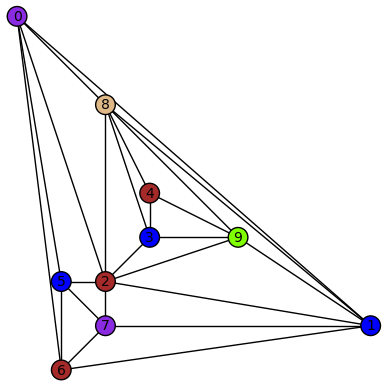
\includegraphics[width=0.6\textwidth]{Images/ListColoring/planar_graph.png}
\end{outImage}


\chapter{Balanced cycle separators in planar graphs}

Let $G$ be a planar triangulation and let $w: F \to \mathbb{R}^+$ be face weight such that $\sum w = 1$ and $w(f) \leq 1/4$ for each face $f$. We would like to find a cycle $C$ in $G$ with property:
$$
\sum_{f \in Int(C)} w(f) \leq 3/4\qquad and \qquad \sum_{f\in Ext(C)} w(f) \leq 3/4
$$
where $Int(C)$ and $Ext(C)$ are interior and exterior faces with respect to the cycle $C$.

\medskip
\noindent Steps of the algorithm are:
\begin{enumerate}
\item Let $T$ be a tree with $\Delta(T) \leq 3$ and let $w: V(T) \to \mathbb{R}^+$ be vertex weight function with $\sum w = 1$ such that $w(v) \leq 1/4$ for each vertex $v$. Then there exist an edge $e$ such that $T - e = T_1 \cup T_2$ and $w(T_1) \leq 3/4$ and $w(T_2) \leq 3/4$. \\
Write function \verb`tree_weight_decomposition(T, w)` which finds such an edge. See hint in the code below for how to do this efficiently!

\item Choose a cycle $C_\infty$ to be the infinite cycle (outer face) and use modified BFS algorithm to find a BFS tree from $C_\infty$ and to determine distance $dist(v)$ from $C_\infty$ for each vertex $v \in V(G)$.

\item Find dual tree $T^*$ of the BFS tree $T$. Vertices of $T^*$ are faces of $G$ and two faces are connected if they are adjacent and the edge between them is not in $T$.

\item Use algorithm from Step 1 to find edge $e^* = (f, g)$ in $T^*$.

\item Find edge $e$ in $G$ which is common edge of faces $f$ and $g$. Then there is a cycle in $T \cup e$. This cycle $C$ is a solution of the algorithm.
\end{enumerate}

\section{Implemetation}

\subsection*{Auxilliary functions}

\begin{sageCell}
    def BFS(G, S):
    import queue

    prev = {}
    dist = {}
    q = queue.Queue()
    for s in S:
        prev[s] = None
        dist[s] = 0
        q.put(s)
    while not q.empty():
        v = q.get()
        for u in G.neighbors(v):
            if u not in prev:
                prev[u] = v
                dist[u] = dist[v] + 1
                q.put(u)
    return prev, dist

def face_edges_to_tuple(F):
    return tuple([u for (u, v) in F])

def tuple_to_face_edges(T):
    """Convert a tuple (a1, a2, ..., ak) representing a face to
    a list of 'edges' [(a1, a2), (a2, a3), ..., (ak, a1)] """
    f = []
    for i in range(len(T)):
        f.append((T[i], T[(i + 1) % len(T)]))
    return f

def face(G):
    """Find one face (sequence of vertices on it); call after embedding is set
    """
    return [a for (a, b) in G.faces()[0]]
\end{sageCell}

\begin{sageCell}
    G = Graph('K{mkXOXC[_{J')  # Planar triangulation
    G.is_planar(set_embedding=True, set_pos=True)  # find planar embedding
    Tr = face(G)  # take the first triangle to be our "initial" triangle
    G.plot(edge_colors={"red": tuple_to_face_edges(Tr)})
\end{sageCell}
\begin{outImage}
   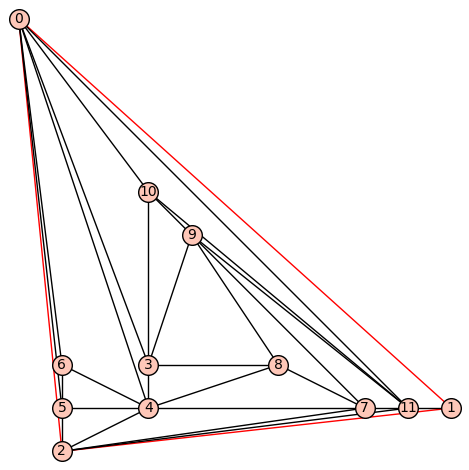
\includegraphics[width=0.6\textwidth]{Images/BalancedSeparators/initial_triangle.png}
\end{outImage}


\subsection*{Step 1}

\begin{sageCell}
def tree_weight_decomposition(T, w):
    """
    Arguments
    T tree, Delta(T) <= 3
    w weights, w: V(T) -> R+, sum w(v) = 1, w(v) <= 1/4

    Result is edge e = (u, v) such that G = T1 + e + T2 and
    w(T1) <= 3/4, w(T2) <= 3/4
    Algorithm should be linear in the number of vertices (edges)
    """
    # See:
    # https://planarity.org/Klein_rooted_forests_and_trees.pdf
    # Lemma 1.3.2
    # Or:
    # Let eweights[(u, v)] be a weight of the component of T - (u, v) containing u
    # Calculate eweights[(u, v)] for each (directed) edge (u, v). You can do this recursively.
    # Find edge e = (u, v) for which difference abs(eweights[(u, v)] - ewighths[(v, u)]) is minimal and return e
    eweights = {}
    mindif = None
    e = None
    for u, v in T.edges(labels = False, sort=False):
        wuv = edge_weight_memo(eweights, T, w, (u, v))
        wvu = edge_weight_memo(eweights, T, w, (v, u))
        if mindif == None or abs(wuv - wvu) < mindif:
            mindif = abs(wuv - wvu)
            e = (u, v)
    return e

def edge_weight_memo(eweights, T, w, e):
    (u, v) = e
    if (u, v) in eweights:
        return eweights[(u, v)]
    else:
        weight = w[u]
        for x in T.neighbors(u):
            if x != v:
                weight += edge_weight_memo(eweights, T, w, (x, u))
        eweights[(u, v)] = weight
        return weight
\end{sageCell}

\section*{Step 2}

\begin{sageCell}
def BFS_graph(G, S):
    """
    G: triangulation,
    S: 'outer' face
    result is pair (T, dist) where is 'tree' from S together with edges of S
    and dist is distance map from S
    """
    prev, dist = BFS(G, S)
    edges = [(u, v) for (u, v) in prev.items() if v != None]
    edges.extend(tuple_to_face_edges(S))
    return Graph(edges), dist
\end{sageCell}

\begin{sageCell}
    BFS_graph(G, Tr)[0].plot()
\end{sageCell}

\begin{outImage}
   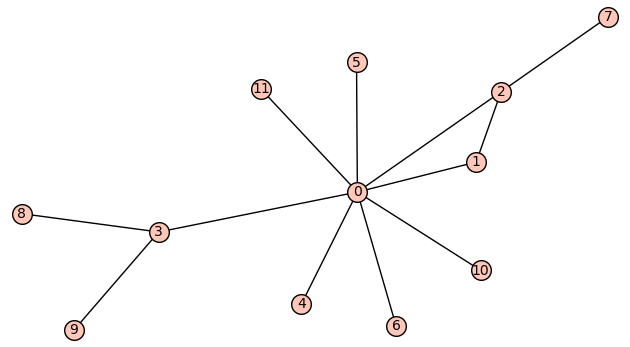
\includegraphics[width=0.6\textwidth]{Images/BalancedSeparators/bfs_tree.png}
\end{outImage}

\begin{sageCell}
    BFS_graph(G, Tr)[1]
\end{sageCell}

\begin{outCell}
    {0: 0, 1: 0, 2: 0, 3: 1, 4: 1, 5: 1, 6: 1, 10: 1, 11: 1, 7: 1, 8: 2, 9: 2}
\end{outCell}
Explanation: dictionary above gives the distances for each vertex from the outer triangle (4, 7, 8)

\section*{Step 3}

\begin{sageCell}
def dual_tree(G, BFSG):
    """Step 3 of the algorithm. Find dual tree. BFSG is the (first) result of the BFS_graph function above
    """
    efaces = G.faces()
    bfsedges = BFSG.edges(labels=False, sort=False)
    edgetoface = {}
    for ef in efaces:
        f = face_edges_to_tuple(ef)
        for u, v in ef:
            edgetoface[(u, v)] = f
    edges = []
    for u, v in G.edges(labels=False, sort=False):
        if (u, v) not in bfsedges and (v, u) not in bfsedges: # lin?
            edges.append((edgetoface[(v, u)], edgetoface[(u, v)]))
    return Graph(edges)
\end{sageCell}

\begin{sageCell}
    dual_tree(G, BFS_graph(G, Tr)[0])
\end{sageCell}
\begin{outImage}
    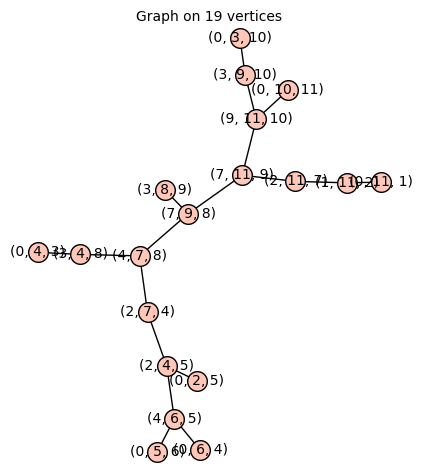
\includegraphics[width=0.6\textwidth]{Images/BalancedSeparators/dual_tree.png}
\end{outImage}
Explanation: Vertices of this graph are faces of the triangulation (except of outer face $(4, 7, 8)$). Two vertices (faces) are connected precisely when the faces are adjacent and the edge between the two faces is not in the BFSG.
For example, faces $(0, 3, 10)$ and $(10, 11, 0)$ are not connected since the edge between them $(0, 10)$ is in the BFSG (see image above), while there is an edge between $(0, 3, 10)$ and $(3, 0, 4)$ since the edge between them $(0, 3)$ is not in BFSG.

\section*{Put everything together}

\begin{sageCell}
def find_cycle_separator(G, S, w):
    BT, dist = BFS_graph(G, Tr)
    DT = dual_tree(G, BT)
    faces = DT.vertices(sort=False)
    finf = tuple(S)
    n = G.num_verts()
    wsum = sum(w.values())

    # Find edge in dual tree
    (fu, fv) = tree_weight_decomposition(DT, w)

    # Find edge in BFS tree
    e = [(u, v) for (u, v) in tuple_to_face_edges(fu) if (v, u) in tuple_to_face_edges(fv)][0]

    # Create cycle
    prev, _ = BFS(BT, [e[0]])
    C = [e[1]]
    while prev[C[-1]] != None:
        C.append(prev[C[-1]])

    return C # , dist, FC, len(faces)
\end{sageCell}
Plot solution:
\begin{sageCell}
    # make uniform weights
    w = dict([(face_edges_to_tuple(f), 1/len(G.faces())) for f in G.faces()])
    C = find_cycle_separator(G, Tr, w)
\end{sageCell}

\begin{sageCell}
    G.plot(edge_colors={"red": tuple_to_face_edges(C)})
\end{sageCell}
\begin{outImage}
    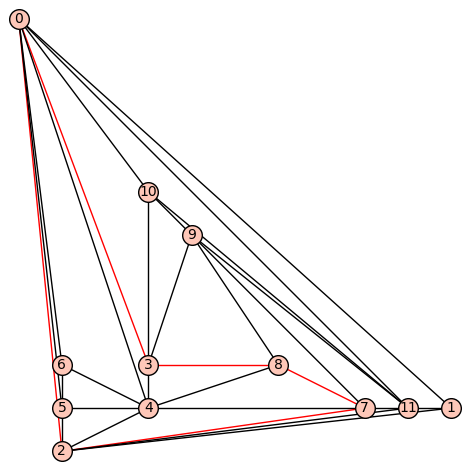
\includegraphics[width=0.6\textwidth]{Images/BalancedSeparators/cycle_separator.png}
\end{outImage}

\begin{sageCell}
    C
\end{sageCell}
\begin{outCell}
    [8, 3, 0, 2, 7]
\end{outCell}
Explanation; the number (since we use uniform weights) of triangles inside and outside red cycle is "balanced", i.e., $\leq 3/4$ of the total number of triangles.


\chapter{Chordal graphs}

\section{Introduction}

A graph $G$ is chordal, if it does not contain an induced cycle of length $\geq 4$. Equivalently, if every cycle $C$ of length $\geq 4$ in $G$ contains a chord.

A \emph{perfect elemination ordering} is an ordering $v_1, v_2, \dots, v_n$ of vertices of $G$ so that $v_i$ is \emph{simplicial vertex} in $G[v_{i}, v_{i+1}, \dots, v_n]$, i.e., $v_i$ and neighbors after it in the ordering form a clique.

A graph $G$ is chordal if and only if it admits a perfect elimination ordering.

\section{Implementation}

\begin{enumerate}
\item Implement \verb`max_cardinality_search(G)` which returns PEO of $G$ using maximal cardinality search algorithm (see \href{http://matematika.fri.uni-lj.si/dm/discrete_mathematics.pdf}{Lecture notes}, Algorithm 7.1.).
\item Write function \verb`is_chordal(G)` which checks if graph $G$ is chordal. Use algorithm 7.2 from Lecture notes. See also comments in the code below.
\item Write function \verb`color_chordal_graph(G)` which returns minimal (optimal) coloring of chordal graph $G$. See Lecture notes.
\end{enumerate}

\begin{sageCell}
def max_cardinality_search(G):
    """
    Maximum cardinality search
    """
    mcs = []
    white = set(G.vertices(sort=False))
    black = set()
    while len(white) > 0:
        maxw = max(white, key = lambda w: len([v for v in G.neighbors(w) if v in black]))
        mcs = [maxw] + mcs
        black.add(maxw)
        white.remove(maxw)
    return mcs

def is_chordal(G):
    """
    Test if graph G is chordal.

    """
    peo = max_cardinality_search(G)
    # We need to check that max_cardinality_search really returns perfect elimination ordering (PEO)
    # let peo be = [v0, v1, ... v{n-1}]
    # for i = 0 ... n-1:
    #    for vi find j > i such that vj is neighbor of vi and j is as small as possible
    #    then, for all vk which are neighbors of vi, k > j, vj and vk must be adjacent
    indexmap = dict(zip(peo, range(len(peo))))
    # v is vi in Algorithm 7.2
    for v in peo:
        # sorted list of peo indexes of "right" neighbors of v
        vnindexes = sorted([indexmap[w] for w in G.neighbors(v) if indexmap[w] > indexmap[v]])
        if len(vnindexes) > 0:
            # u is the first "right" neighbor of v in peo (vj in Algorithm 7.2)
            u = peo[vnindexes[0]]
            for wi in vnindexes[1:]:
                if not G.has_edge(u, peo[wi]):
                    return False
    return True

def color_chordal_graph(G):
    """
    Optimally color chordal graph G.
    """
    col = {}
    peo = max_cardinality_search(G);
    # Algorithm is greedy and efficient:
    #   go from the last to the first vertex in peo
    #   select the first available color for v (smallest not used by right neighbors)
    # Thus, for chordal graphs optimal coloring is "easy" problem!
    indexmap = dict(zip(peo, range(len(peo))))
    colors = range(len(peo))
    # go from the last to the first vertex in peo
    for v in reversed(peo):
        # colors of right neighbors
        vncol = set([col[w] for w in G.neighbors(v) if indexmap[w] > indexmap[v]])
        # select the first available color for v (smallest not used by right neighbors)
        col[v] = next(enumerate(c for c in colors if c not in vncol))[1]
    return col
\end{sageCell}

\subsection*{Examples}

\begin{sageCell}
def random_chordal_graph(n, kmin = 5, kmax = 10, kidmin = 2, kidmax = 4):
    """Returns a 'random' chordal graph.
    The sizes of maximal cliques are between `kmin` and `kmax`,
    the intersections of maximal cliques are between `kidmin` and `kidmax`."""
    from random import randint, sample

    G = Graph()
    cliques = []
    nG = 0

    # create cliques
    for i in range(n):
        s = randint(kmin, kmax)
        K = graphs.CompleteGraph(s)
        K.relabel(lambda w: w + nG)
        G = G.union(K)
        cliques.append(K.vertices(sort=False))
        nG += s

    # merge parts of cliques
    for i in range(1, n):
        j = randint(0, i - 1)
        C1 = cliques[j]
        C2 = cliques[i]
        nmin = min(len(C1), len(C2))
        k = randint(kidmin, min(kidmax, nmin - 1))
        iC1 = sample(C1, k)
        iC2 = sample(C2, k)
        id = zip(iC1, iC2)
        for (u, v) in id:
            G.merge_vertices((u, v))
            C2 = [u if x == v else x for x in C2]
        cliques[i] = C2
    return G
\end{sageCell}

\begin{sageCell}
    def apollonian_network(n):
    """Apollonian network is a graph formed by a process of recursively subdividing a triangle
    into three smaller triangles. This function returns Apollonian network on n vertices, n >= 3."""
    from random import choice
    G = graphs.CycleGraph(3)
    pos = {0: [1, 0], 1: [-0.5, 0.866], 2: [-0.5, -0.866]}
    faces = [[0, 1, 2]]
    for i in range(3, n):
        f = choice(faces)
        x, y, z = f
        faces.remove(f)
        faces.extend([[x, y, i], [i, y, z], [i, z, x]])
        G.add_edges([(x, i), (y, i), (z, i)])
        xi = sum(a for (a, b) in [pos[w] for w in [x, y, z]])/3
        yi = sum(b for (a, b) in [pos[w] for w in [x, y, z]])/3
        pos[i] = (xi, yi)
    G.set_pos(pos)
    return G
\end{sageCell}

\begin{sageCell}
    G = random_chordal_graph(3)
    max_cardinality_search(G), is_chordal(G)
\end{sageCell}
\begin{outCell}
    ([22, 19, 17, 16, 15, 14, 13, 8, 7, 6, 5, 4, 3, 2, 1, 0], True)
\end{outCell}

\begin{sageCell}
    is_chordal(graphs.CompleteGraph(4))
\end{sageCell}
\begin{outCell}
    True
\end{outCell}

\begin{sageCell}
    is_chordal(graphs.CycleGraph(4))
\end{sageCell}
\begin{outCell}
    False
\end{outCell}

\begin{sageCell}
def color_graph(G, coloring, **kwargs):
    all_colors = list(colors)[10:];
    color_map = {}
    for v, c in coloring.items():
        color = all_colors[c]
        color_map.setdefault(color, []).append(v)
    return G.plot(vertex_colors=color_map, **kwargs)
\end{sageCell}
\begin{sageCell}
    G = apollonian_network(10)
    coloring = color_chordal_graph(G)
    color_graph(G, coloring)
\end{sageCell}

\begin{outImage}
   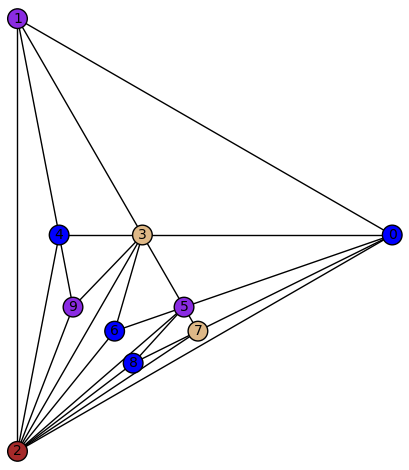
\includegraphics[width=0.6\textwidth]{Images/ChordalGraphs/apollonian_network.png}
\end{outImage}



\chapter{Tree decomposition}

A \emph{tree decomposition} of a (connected) graph $G$ is a tree $T$ such that
\begin{enumerate}
    \item each vertex $v$ of the graph $G$ is contained in a vertex (bag) of $T$,
    \item for each edge $uv$ of the graph $G$, there is a vertex (bag) of $T$ that contains both $u$ and $v$,
    \item for each vertex $v$ of $G$, the set of vertices of $T$ which contain $v$ induce a connected subtree.
\end{enumerate}

\section{Exercises}

\subsection{Bucket elimination}

Bucket elimination is a heuristic algorithm for finding a tree decomposition for a graph $G$.

\medskip
\noindent \textbf{Algorithm:}
Order the vertices of $G$ by non-increasing degree
\begin{enumerate}
    \item for each vertex $v \in V(G)$ add a vertex to $T$ with the initial bag $B(v)$ containing $v$,
    \item for each edge $uv \in E(G)$ add the "left" vertex to the bag of the "right" vertex,
    \item From right to left process the vertices $v$:
    \begin{enumerate}
        \item let $A$ be the bag $B(v) \setminus \{v\}$,
        \item let $u$ be the rigthmost vertex in $A$,
        \item add $A$ to the bag $B(u)$ and add  edge $uv$ to the tree.
    \end{enumerate}
\end{enumerate}

Write a function \verb`bucket_elimination(G)` which returns a tree decomposition of $G$ computed by the bucket elimination algorithm.
Also, write a function \verb`decomposition_width(B)` which returns the width of the tree decomposition $B$, $B$ is a bucket map returned by the function \verb`bucket_elimination`. Compare with the value returned by the Sage function \verb`treewidth()`.

\subsubsection*{Solution and tests}
\begin{sageCell}
def bucket_elimination(G):
    """
    Bucket elimination algorithm for finding a tree decomposition of a graph G.
    Returns a tree decomposition T and a bucket map B (dictionary with bags for each vertex of T).
    """
    T = Graph()
    B = {}
    vrt = sorted(G.vertices(sort=False), key=G.degree, reverse=True)
    T.add_vertices(vrt)
    for x in vrt:
        B[x] = set([x])

    for x, y in G.edges(labels=False, sort=False):
        if vrt.index(x) < vrt.index(y):
            B[y] = B[y] | set([x])
        else:
            B[x] = B[x] | set([y])

    for x in reversed(vrt):
        A = copy(B[x])
        A.remove(x)
        if len(A) > 0:
            y = max(A, key=lambda z: vrt.index(z))
            T.add_edge((x, y))
            B[y] = B[y] | A

    return T, B
\end{sageCell}

\begin{sageCell}
def decomposition_width(B):
    return max(len(B[x]) for x in B) - 1
\end{sageCell}
Example
\begin{sageCell}
    G = Graph('S?G?KG?Ax`????CPG?Q??Cp_@?GOAG?P?')
    G.plot()
\end{sageCell}
\begin{outImage}
    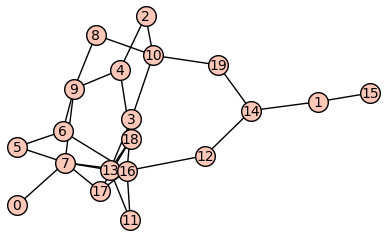
\includegraphics[width=0.5\textwidth]{Images/TreeDecomposition/bucket_elimination_graph.png}
\end{outImage}

\begin{sageCell}
    T, B = bucket_elimination(G)
\end{sageCell}
\begin{sageCell}
    T.plot()
\end{sageCell}
\begin{outImage}
   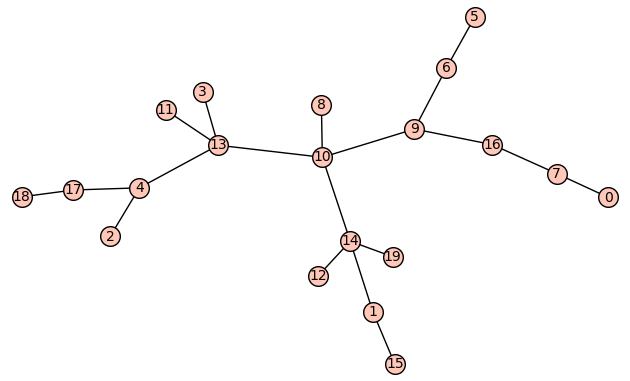
\includegraphics[width=0.5\textwidth]{Images/TreeDecomposition/bucket_elimination.png}
\end{outImage}

\begin{sageCell}
    B
\end{sageCell}
\begin{outCell}
    {7: {7},
     16: {7, 16},
     9: {7, 9, 16},
     10: {7, 9, 10, 16},
     13: {7, 9, 10, 13, 16},
     3: {3, 10, 13, 16},
     4: {4, 7, 9, 10, 13, 16},
     6: {6, 7, 9, 16},
     14: {10, 14, 16},
     17: {4, 7, 13, 16, 17},
     18: {4, 13, 17, 18},
     1: {1, 14},
     2: {2, 4, 10},
     5: {5, 6, 7},
     8: {8, 9, 10},
     11: {11, 13, 16},
     12: {12, 14, 16},
     19: {10, 14, 19},
     0: {0, 7},
     15: {1, 15}}
\end{outCell}

\begin{sageCell}
    decomposition_width(B)
\end{sageCell}
\begin{outCell}
    5
\end{outCell}
The result is 5, the size of the largest bucket $-1$

Compare to the built-in function returning tree width (should get less or equal than by \verb`decomposition_width`)
\begin{sageCell}
    T.treewidth()
\end{sageCell}
\begin{outCell}
    4
\end{outCell}


\subsection{Nice tree decomposition}

A \emph{nice tree decomposition} is a rooted binary tree decomposition with four kinds of tree vertices:
\begin{enumerate}
    \item \textbf{start}: leaves have bags of size 1,
    \item \textbf{introduce}: a vertex $v$ with one child $u$, the bag of $u$ contains one element less than the bag of $v$,
    \item \textbf{forget}:  a vertex $v$ with one child $u$, the bag of $u$ contains one element more than the bag of $v$,
    \item \textbf{join}: a vertex $v$ with two children, both have the same bag as $v$.
\end{enumerate}
Write function \verb`nice_tree_decomposition(G, T, B)` which transforms the tree decomposition $(T, B)$ of the graph $G$ into a "nice tree decomposition".

\subsubsection*{Solution and tests}


Auxiliary functions
\begin{sageCell}
    def DDFS(T, r):
    """Directs the tree T to the root r."""
    active = [r]
    prev = {}
    while len(active) > 0:
        v = active.pop()
        for w in T.neighbors(v):
            if w not in prev and w not in active and w != r:
                prev[w] = v
                active.append(w)
    DT = DiGraph()
    DT.add_edges(prev.items())
    return DT
\end{sageCell}

\begin{sageCell}
def nice_tree_decomposition(T, B):
    T = T.copy()
    B = dict((v, copy(b)) for (v, b) in B.items())
    ntd_handle_leaves(T, B)
    ntd_handle_edges(T, B)
    r = T.vertices(sort=False)[0]
    DT = DDFS(T, r)
    ntd_handle_multiple_children(DT, B)
    return DT, B

def new_vertex(G):
    """Returns integer v such that v, v + 1, v + 2, ... can be used as new vertices in G."""
    vrt = [0] + [x for x in G.vertices(sort=False) if type(x) == type(1) or type(x) == type(int(1))]
    return max(vrt) + 1

def ntd_handle_leaves(T, B):
    """
    If a leaf has a bag of size > 1, then we add a new leaf with a bag with one element less and repeat until all leaves have bags of size 1.
    """
    leaves = [x for x in T.vertices(sort=False) if T.degree(x) == 1]
    nv = new_vertex(T)

    for l in leaves:
        A = copy(B[l])
        while len(A) > 1:
            T.add_edge((l,nv))
            A.pop()
            B[nv] = copy(A)
            l = nv
            nv = nv + 1

def ntd_handle_edges(T, B):
    nv = new_vertex(T)

    for (x, y) in T.edges(labels=False, sort=False):
        Bx = copy(B[x])
        By = copy(B[y])
        Bxy = Bx & By

        if len(By) < len(Bx):
            x, y = y, x
            Bx, By = By, Bx

        T.delete_edge((x, y))

        path = [a for a in Bx if a not in Bxy]
        while path != []:
            a = path.pop()
            T.add_edge((x, nv))
            Bx.remove(a)
            B[nv] = copy(Bx)
            x = nv
            nv = nv + 1

        path = [a for a in By if a not in Bxy]
        path.pop()
        while path != []:
            a = path.pop()
            T.add_edge((x, nv))
            Bx = Bx | set([a])
            B[nv] = copy(Bx)
            x = nv
            nv = nv + 1
        T.add_edge((x, y))

def ntd_handle_multiple_children(DT, B):
    big_vertices = [x for x in DT.vertices(sort=False) if DT.in_degree(x) > 2]
    nv = new_vertex(DT)

    while big_vertices != []:
        v = big_vertices.pop()
        Nv = DT.neighbors_in(v)
        Nv.pop()
        for u in Nv:
            DT.delete_edge((u, v))
            DT.add_edge((u, nv))
        DT.add_edge((nv, v))
        B[nv] = copy(B[v])
        if len(Nv) > 2:
            big_vertices.append(nv)
        nv = nv + 1

    big_vertices = [x for x in DT.vertices(sort=False) if DT.in_degree(x) == 2]
    for v in big_vertices:
        u,w = DT.neighbors_in(v)
        if B[u] != B[v]:
            DT.delete_edge((u, v))
            DT.add_path((u, nv, v))
            B[nv] = copy(B[v])
            nv = nv + 1
        if B[w] != B[v]:
            DT.delete_edge((w, v))
            DT.add_path((w, nv, v))
            B[nv] = copy(B[v])
            nv = nv + 1
\end{sageCell}
Example
\begin{sageCell}
    NT, NB = nice_tree_decomposition(T, B)
\end{sageCell}

\begin{sageCell}
def is_nice_tree_decomposition(G, T, B):
    if not is_tree_decomposition(G, T, B):
        return False
    for v in T.vertices(sort=False):
        nin = NT.neighbors_in(v)
        if len(nin) == 0: # leaf
            if len(B[v]) != 1:
                print(f"leaf {v} has bag of size {len(B[v])}")
                return False
        elif len(nin) > 2:
            print(f"vertex {v} has 3 or more children")
        elif len(nin) == 1:
            u = nin[0]
            ints = B[v] & B[u]
            if len(B[v] - ints) > 1 or len(B[u] - ints) > 1:
                print(f"verices {v} and {u} have bags {B[v]} and {B[u]} with difference > 1")
        # len(nin) == 2
        elif B[v] != B[nin[0]] or B[v] != B[nin[1]]:
            print(f"children of {v} have different bags")
            return False
    return True
\end{sageCell}

\begin{sageCell}
    is_nice_tree_decomposition(G, NT, NB)
\end{sageCell}
\begin{outCell}
    True
\end{outCell}



\chapter{Maximum independent set}

Write a function \verb`max_independent_set(G, T, B)` which computes a maximum independent set of a graph $G$ with a nice tree decomposition $(T, B)$ (see previous chapter). Algorithm should perform well on graphs with small tree width.

\subsection*{Solution}

\begin{sageCell}
def max_independent_set(G, DT, r, B):
    """Returns maximal independent set of graph G with nice tree decomposition DT, r, B (directed tree with root r and
    bucket map B)"""
    maxI = None
    MEM = {}  # Memorize all results of max_independent_set_rec
    # Dictionary of independent sets for all bags
    rsets = independent_sets(G, B[r])
    # Take maximum over all possible independent sets of the root bag
    for S in rsets:
        IS = max_independent_set_rec(G, DT, B, r, S, MEM)
        if IS != None:
            if maxI == None or len(IS) > len(maxI):
                maxI = IS
    return maxI

def max_independent_set_rec(G, DT, B, t, S, MEM):
    """Returns the largest independent set of the subgraph of G induced on bags below (including) t
    which contains all vertices from S (More precisely, vertices of this independent set from B[t] are exactly vertices S).
    Parameters:
      G        graph
      (DT, B)  tree decomposition with tree directed towards the root
      t        tree vertex
      S        a independent set of bag B[t]"""
    if (t, tuple(S)) in MEM:
        return MEM[(t, tuple(S))]  # If we already calculated the result
    result = None
    sons = DT.neighbors_in(t)
    Bt = B[t]
    if len(sons) == 0: # leaf, len(Bt) == 1
        return S
    elif len(sons) == 1:
        s = sons[0]
        Bs = B[s]
        if len(Bs) > len(Bt): # t is forget node
            u = list(Bs - Bt)[0]  # len(diff) = 1
            result = max_independent_set_rec(G, DT, B, s, S, MEM)
            Su = S | set([u])
            if is_independent_set(G, Su):
                result2 = max_independent_set_rec(G, DT, B, s, Su, MEM)
                if len(result2) > len(result):
                    result = result2
        else: # len(Bs) < len(Bt) - t is introduce node
            u = list(Bt - Bs)[0]  # len(diff) = 1
            Su = S - set([u])
            result = max_independent_set_rec(G, DT, B, s, Su, MEM)
    elif len(sons) == 2:  # join node
        s1 = sons[0]
        s2 = sons[1]
        result1 = max_independent_set_rec(G, DT, B, s1, S, MEM)
        result2 = max_independent_set_rec(G, DT, B, s2, S, MEM)
        result = result1 | result2
    else:
        # should not happen
        return None
    result = result | S
    MEM[(t, tuple(S))] = result  # Memorize the result
    return result
\end{sageCell}
Auxilliary function:
\begin{sageCell}
def independent_sets(G, X):
    """Returns all independent sets of the subgraph of G induced on the set X; exhaustive search, suitable for small X"""
    if len(X)==0:
        return [set([])]
    else:
        X1 = copy(X)
        X2 = copy(X)
        v = X1.pop()
        X2.remove(v)
        Nv = [w for w in G.neighbors(v) if w in X]
        for w in Nv:
            X2.remove(w)
        C1 = independent_sets(G, X1)
        C2 = independent_sets(G, X2)
        C2 = [i.union([v]) for i in C2]
        return C1 + C2
\end{sageCell}

\subsection*{Tests}

\begin{sageCell}
def is_independent_set(G, X):
    return G.subgraph(X).num_edges() == 0
\end{sageCell}

\begin{sageCell}
    G1 = Graph('XTnNw?DOYHgJ@BP@g`wG^PAoa?@C?G??Ga?EG_@oC?NcO?}???P')
    T1, r1, B1 = nice_tree_decomposition(G1)
    MI1 = max_independent_set(G1, T1, r1, B1)
    (is_independent_set(G1, MI1), len(MI1)) == (True, 7)
\end{sageCell}
\begin{outCell}
    True
\end{outCell}



\chapter{Matchings and covers in bipartite graphs}

Given a graph $G = (V,E)$, a \emph{matching} $M$ in $G$ is a set of pairwise non-adjacent edges; that is, no two edges share a common vertex. A \emph{maximum matching} is a matching that contains the largest possible number of edges.

A (\emph{vertex}) \emph{cover} $C$ in $G$ is a set of vertices such that for every edge $uv \in E$, either $u \in C$ or $v \in C$. A \emph{minimum cover} is a cover of the smallest possible size.

\subsection*{Algorithm for bipartite graphs}

Maximum matching (and minumum cover) in bipartite graphs can be found in polynomial time using Max-Flow-Min-Cut algorithm (Ford Fulkerson).

\medskip
\noindent \textbf{Algorithm:}
\begin{enumerate}
\item Let $G$ be a bipartite graph with vertex bipartition $V(G) = A \cup B$.
\item Create a directed weighted graph $G^+$ with vertex set $V(G) \cup \{s, t\}$, i.e., add two vertices, source ($s$) and sink ($t$).
\item Edges of $G^+$ are edges $(s, a)$, $a \in A$, $(b, t)$, $b \in B$ and edges of the original graph directed from $A$ to $B$.
\item Put weight (capacity) $1$ to edges of type $(s, a)$ and $(b, t)$ and $\infty$ (a large integer, e.g., the number of vertices in $G$) to all other edges (edges between $A$ and $B$).
\item Compute (integer) max flow $f$ with source $s$ and sink $t$.
\item Maximum matching consist of edges $\{uv \in E(G) \mid f(u, v) = 1\}$.
\item Compute min cut $(S, T)$, such that $s \in S$ and $t \in T$.  Minimum cover of $G$ is set $C = \{v \in A \mid v \in T\} \cup \{v \in B \mid v \in S\}$
\end{enumerate}

\medskip
\noindent Why does this algortihm work?

\medskip
Let $f$ be the max flow (integral!) obtained in 5. Then the edge set in 6 is clearly a matching, since flow "coming" from the vertex $s$ to a vertex $a \in A$ has value 1 and, since it is integral, cannot "split" from $a$ towards two vertices in $B$ Also flow cannot "come" to a vertex $b \in B$ from two vertices in $A$, since it is integral and capacity of the edge $(b, t)$ is 1.

The reverse is also true, any matching $M$ produces a flow from $s$ to $t$ with value $|M|$. Therefore a max flow gives a max matching and a max matching gives a max flow.

What about min cut. The set $C$ from 7 is a cover, since every edge with endpoint in $A \cap T$ is covered and also every edge with endpoint in $B \cap S$ is covered. The only uncovered edges would be edges between $A \cap S$ and $B \cap T$, but that edges would be part of the cut, and since their capacity is infinity, min cut would have infinite value. This is clearly not possible since a trivial cut $S = \{s\}, T = A \cup B \cup \{t\}$ is clearly finite ($|A|$). The other way is also easy to see. For every cover of $G$ you can construct a cut of $G^+$ of the form in 7. See this (http://\url{www.cs.toronto.edu/~siavosh/csc373h/files/TN6.pdf} for more detailed explanation.

\subsection{Exercise}

Write functions \verb`max_bipartite_matching(G)` and \verb`min_bipartite_cover(G)` which return maximum matching and minimum cover in bipartite graph $G$. You can use Sage functions \href{http://doc.sagemath.org/html/en/reference/graphs/sage/graphs/generic_graph.html#sage.graphs.generic_graph.GenericGraph.flow}{flow} and \href{http://doc.sagemath.org/html/en/reference/graphs/sage/graphs/generic_graph.html#sage.graphs.generic_graph.GenericGraph.edge_cut}{edge cut} to obtain max flow and min cut, respectively.

\subsubsection*{Maximum bipartite matching}
\begin{sageCell}
def max_bipartite_matching(G):
    A, B = G.bipartite_sets()
    Gp = DiGraph()
    Gp.add_vertices(G.vertices())
    s = Gp.add_vertex()
    t = Gp.add_vertex()
    Gp.add_edges([(s, a, 1) for a in A])
    Gp.add_edges([(b, t, 1) for b in B])
    for a in A:
        Gp.add_edges([(a, b, G.num_verts()) for b in G.neighbors(a)])
    val, flow = Gp.flow(s, t, integer=True, value_only=False)
    return [(u, v) for (u, v) in flow.edges(labels = False) if (u != s and v != t)]
\end{sageCell}
Example:
\begin{sageCell}
    G = Graph({1: [5, 6, 8], 2: [5, 7], 3: [7], 4: [7]})
    G.set_pos({1: (0, 1), 2: (0, 2), 3: (0, 3), 4: (0, 4), 5: (1, 1), 6: (1, 2), 7: (1, 3), 8: (1, 4)})
    G.plot()
\end{sageCell}
\begin{outImage}
    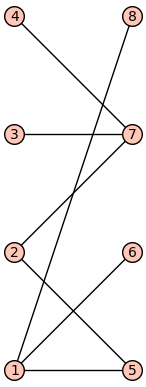
\includegraphics[width=0.15\textwidth]{Images/BipartiteMatchings/bipartite_graph.png}
 \end{outImage}
\begin{sageCell}
    G.bipartite_sets()
\end{sageCell}
\begin{outCell}
    ({1, 2, 3, 4}, {8, 5, 6, 7})
\end{outCell}
\begin{sageCell}
    max_bipartite_matching(G)
\end{sageCell}
\begin{outCell}
    [(1, 6), (2, 5), (3, 7)]
\end{outCell}
\begin{sageCell}
    G.show(edge_colors={"red": max_bipartite_matching(G)})
\end{sageCell}
\begin{outImage}
    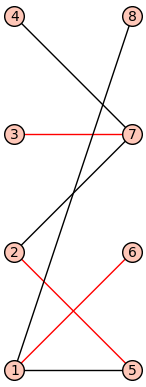
\includegraphics[width=0.15\textwidth]{Images/BipartiteMatchings/bipartite_graph_matching.png}
 \end{outImage}

 \subsubsection*{Minimum bipartite cover}

\begin{sageCell}
def min_bipartite_cover(G):
    A, B = G.bipartite_sets()
    Gp = DiGraph()
    Gp.add_vertices(G.vertices())
    s = Gp.add_vertex()
    t = Gp.add_vertex()
    Gp.add_edges([(s, a, 1) for a in A])
    Gp.add_edges([(b, t, 1) for b in B])
    for a in A:
        Gp.add_edges([(a, b, G.num_verts()) for b in G.neighbors(a)])
    _, _, sets = Gp.edge_cut(s, t, vertices=True)
    return [v for v in A if v in sets[1]] + [v for v in B if v in sets[0]]
\end{sageCell}
Example:
\begin{sageCell}
    G.show(vertex_colors={"red": min_bipartite_cover(G)})
\end{sageCell}
\begin{outImage}
    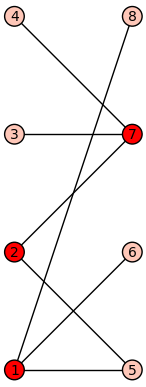
\includegraphics[width=0.15\textwidth]{Images/BipartiteMatchings/bipartite_graph_cover.png}
\end{outImage}




\chapter{Stable matchings}

\section{Introduction}

Write function \verb`stable_matchings(F, M)`' which implements stable matchings algorithm. $F$ is a dictionary of priority lists of women and $M$ is a dictionary of priority lists of men. It should return a list of "matching" pairs (female, male).

\medskip
\noindent \textbf{Algorithm:}
\begin{verbatim}
while exists a woman f who is not engaged and has not proposed
to all men do:
    f proposes to her best candidate m, whom she has not yet proposed to;
    if m is not engaged then
        f and m engage to be married
    else if m prefers f to his current fiancee f' then
        f' and m break up their engagement
        f and m engage to be married
    return M
\end{verbatim}

\section{Implementation}

\begin{sageCell}
def stable_matchings(F, M):
    """
    F is a dictionary woman -> list of men sorted by the priorities
    M is a dictionary man -> list of women sorted by the priorities
    return a list of matching pairs (f, m)
    """
    FL = dict([(f, l[:]) for (f, l) in F.items()]) # for every woman a list of men left to propose, sorted by priority
    ML = dict([(m, l[:]) for (m, l) in M.items()])
    unmatchedF = list(FL.keys())
    FM = {}
    MM = {}
    while len(unmatchedF) > 0:
        f = unmatchedF.pop(0)
        fL = FL[f]
        if len(fL) == 0:
            continue
        m = fL.pop(0)
        if not m in MM:
            MM[m] = f
            FM[f] = m
        elif ML[m].index(f) < ML[m].index(MM[m]):
            fx = MM[m]
            MM[m] = f
            FM[f] = m
            del FM[fx]
            unmatchedF.append(fx)
        else:
            unmatchedF.append(f)
    return list(FM.items())
\end{sageCell}

\begin{sageCell}
def is_matching_stable(match, F, M):
    for f, m in match:
        fList = F[f]
        mi = fList.index(m)
        for i in range(0, mi):
            altm = fList[i]
            altmList = M[altm]
            altmCurrent = next(f for (f, m) in match if m == altm)
            altmCurrentRank = altmList.index(altmCurrent)
            altmFRank = altmList.index(f)
            if altmFRank < altmCurrentRank:
                print(f"Pair {f}-{m} is not stable, {f}-{altm} violates stable marriage condition")
                return False
    return True
\end{sageCell}

\begin{sageCell}
    F = {1: [4, 1, 3, 2], 2: [3, 1, 2, 4], 3: [4, 3, 2, 1], 4: [4, 3, 2, 1]} # e.g, woman 1 prefers man 4 over all other men (he is the first in her list)
    M = {1: [2, 3, 1, 4], 2: [4, 3, 1, 2], 3: [1, 2, 3, 4], 4: [1, 2, 3, 4]} # e.g, man 1 prefers woman 2 over all other women (she is the first in his list)
\end{sageCell}

\begin{sageCell}
    match = stable_matchings(F, M)
    match
\end{sageCell}
\begin{outCell}
    [(1, 4), (2, 3), (4, 2), (3, 1)]
\end{outCell}

\begin{sageCell}
    is_matching_stable(match, F, M)
\end{sageCell}
\begin{outCell}
    True
\end{outCell}

\begin{sageCell}
    is_matching_stable([(1, 2), (2, 3), (4, 4), (3, 1)], F, M)
\end{sageCell}
Pair 1-2 is not stable, 1-4 violates stable marriage condition
\begin{outCell}
    False
\end{outCell}


%------------------------------------------------

\chapter*{Bibliography}

\markboth{\sffamily\normalsize\bfseries Bibliography}{\sffamily\normalsize\bfseries Bibliography} % Set the page headers to display a Bibliography chapter name
\addcontentsline{toc}{chapter}{\textcolor{ocre}{Bibliography}} % Add a Bibliography heading to the table of contents

\section*{Articles}
\addcontentsline{toc}{section}{Articles} % Add the Articles subheading to the table of contents

\printbibliography[heading=bibempty, type=article] % Output article bibliography entries

\section*{Books}
\addcontentsline{toc}{section}{Books} % Add the Books subheading to the table of contents

\printbibliography[heading=bibempty, type=book] % Output book bibliography entries

\end{document}
